\documentclass[11pt]{article}
\usepackage{mathblatt}


\begin{document}
\pfheftstil
\pfheftkopf{Kurvenuntersuchung}{Abi GK}
\pfrueckblick
\begin{pfaufg}{}{1.}{}
Ein Getränk wird in einen Raum mit $20$ °C gebracht. Die Abbildung zeigt seine Temperatur $T$ (in °C) $t$ Minuten danach. Beschreibe den Verlauf im Sachzusammenhang.
\par\smallskip\noindent \begin{ksys}[xmin=0,xmax=40,ymin=0,ymax=100,xstep=10,ystep=20,xlabel=t in min,ylabel=T in °C,ablesen] \funktionab{20+40*exp(-0.1*\x)}{T}{0}{40} \end{ksys}\par
\rechenplatz{1}
\end{pfaufg}
\begin{pfaufg}{}{2.}{}
Gegeben ist die Ableitung $f'(x) = 2x - 6$. Bestimme das Vorzeichen von $f'(x)$ auf dem Intervall $[0; 2]$ und kreuze an. 
\pfkreuzzeile{$f$ steigt auf diesem Intervall}\pfkreuzzeile{$f$ fällt auf diesem Intervall}
\end{pfaufg}
\pfstufekopf[snullstellenundachsen]{Nullstellen und Achsenschnittpunkte berechnen}{in 5 der letzten 5 Prüfungen}
\pfgruppe{Was ist zu tun? Ankreuzen, nicht rechnen}
\begin{pfaufg}{}{3.}{}
$f(x) = (x + 4)(x - 7)$ – welches Verfahren? 
\pfkreuzzeile{Faktoren null setzen}\pfkreuzzeile{ausklammern}\pfkreuzzeile{substituieren}\pfkreuzzeile{Polynomdivision}\pfkreuzzeile{Lösungsformel}
\fusshilfe{\mbox{3:~Faktoren null setzen}}
\end{pfaufg}
\begin{pfaufg}{}{4.}{}
Wie hoch ist der Ball $2$ s nach dem Abwurf? – Wert oder Stelle? 
\pfkreuzzeile{Stelle gegeben, Wert gesucht}\pfkreuzzeile{Wert gegeben, Stelle gesucht}
\fusshilfe{\mbox{4:~Stelle gegeben, Wert gesucht}}
\end{pfaufg}
\pfgruppe{}
\begin{pfaufg}{}{5.}{}
$f(x) = x^3 - x^2 - 6x$ – alle Schnittpunkte mit den Achsen?
\rechenplatz{2}
\fusshilfe{\mbox{5:~$N_1(-2 | 0)$, $N_2(0 | 0)$, $N_3(3 | 0)$}}
\end{pfaufg}
\pfgruppe{}
\begin{pfaufg}{Abi ’25\\ohne Hilfsmittel}{6.}{1 BE}
Gegeben ist die in $\mathbb{R}$ definierte Funktion $f$ mit $f(x) = 2e^x - 2e$; die Abbildung zeigt ihren Graphen. Weise nach, dass 1 eine Nullstelle von $f$ ist.
\par\smallskip\noindent \begin{tikzpicture}\begin{axis}[xmin=-4.0,xmax=2.0,ymin=-6.0,ymax=2.0,axis lines=middle,width=11cm,height=7cm,xlabel={$x$},ylabel={$y$},tick label style={font=\scriptsize},samples=160,clip=true,every axis plot/.append style={line width=0.9pt},/pgf/number format/use comma,grid=both,grid style={mbgitter},minor tick num=1]\addplot[black,domain=-4.0:2.0] {2*exp(x)-2*2.718281828};\node[font=\small,fill=white,inner sep=1pt,anchor=south west] at (axis cs:1.04,{2*exp((1.04))-2*2.718281828}) {$G_f$};\end{axis}\end{tikzpicture}\par
\rechenplatz{1}
\fusshilfe{\mbox{6:~f(1) = 2e $-$ 2e = 0}}
\end{pfaufg}
\pfgruppe{}
\begin{pfaufg}{Abi ’26}{7.}{1 BE}
Ein Speicherofen kühlt ab. Die Temperatur seiner Oberfläche in °C wird beschrieben durch $k(x) = 60e^{-\tfrac{x}{400}} + 20$; $x$ ist die Zeit in Minuten seit Beginn des Abkühlens. Gib die Temperatur zu Beginn an.
\rechenplatz{1}
\fusshilfe{\mbox{7:~80 °C}}
\end{pfaufg}
\pfgruppe{}
\begin{pfaufg}{Abi ’22\\ohne Hilfsmittel}{8.}{2 BE}
Berechne die Nullstellen der Funktion $f$ mit $f(x) = x^3 - 8x^2 + 12x$.
\rechenplatz{2}
\fusshilfe{\mbox{8:~x = 0, x = 2, x = 6}}
\end{pfaufg}
\pfgruppe{}
\begin{pfaufg}{Abi ’26}{9.}{3 BE}
Gegeben ist die Funktion $f$ mit $f(x) = 3e^x + 1$, $x \in \mathbb{R}$; ihr Graph heißt $G_f$. Begründe am Funktionsterm, dass $G_f$ die $x$-Achse nicht schneidet. Gib die Wertemenge von $f$ an.
\par\smallskip\noindent \begin{tikzpicture}\begin{axis}[xmin=-3.0,xmax=2.0,ymin=0.0,ymax=6.0,axis lines=middle,width=11cm,height=7cm,xlabel={$x$},ylabel={$y$},tick label style={font=\scriptsize},samples=160,clip=true,every axis plot/.append style={line width=0.9pt},/pgf/number format/use comma,grid=both,grid style={mbgitter},minor tick num=1]\addplot[black,domain=-3.0:2.0] {3*exp(x)+1};\node[font=\small,fill=white,inner sep=1pt,anchor=south west] at (axis cs:0.30000000000000027,{3*exp((0.30000000000000027))+1}) {$G_f$};\end{axis}\end{tikzpicture}\par
\rechenplatz{2}
\fusshilfe{\mbox{9:~Wertemenge ]1}}
\end{pfaufg}
\pfgruppe{}
\begin{pfaufg}{Abi ’23}{10.}{4 BE}
Gegeben ist die Funktion $f$ mit $f(x) = x^3 - 12x^2 + 45x - 50$, $x \in \mathbb{R}$. Man kann den Term auch als $f(x) = (x - 5)\cdot(x^2 - 7x + 10)$ schreiben. Gib die Koordinaten des Punkts an, in dem der Graph von $f$ die $y$-Achse schneidet. Ermittle, wie viele Nullstellen $f$ hat.
\rechenplatz{3}
\fusshilfe{\mbox{10:~(0 | $-$50); 5}}
\end{pfaufg}
\pfgruppe{}
\begin{pfaufg}{Abi ’24}{11.}{4 BE}
Gegeben ist die Funktion $f$ mit $f(x) = 0{,}5x^4 - 4x^2 + 3{,}5$, $x \in \mathbb{R}$; ihr Graph heißt $G_f$. Gegeben: $G_f$ ist achsensymmetrisch zur $y$-Achse, und $(1 \mid 0)$ liegt auf $G_f$. Begründe ohne Rechnung, dass auch $(-1 \mid 0)$ auf $G_f$ liegt. Bestimme die übrigen Schnittpunkte von $G_f$ mit der $x$-Achse.
\rechenplatz{3}
\fusshilfe{\mbox{11:~($-$1 | 0) wegen Achsensymmetrie}}
\end{pfaufg}
\pfgruppe{}
\begin{pfaufg}{Abi ’24}{12.}{2 BE}
Gegeben ist die in $\mathbb{R}$ definierte Funktion $f$ mit $f(x) = (x - 2)\cdot e^{-\tfrac{x}{2} + 3}$ und ihrer Ableitung $f'(x) = \left(-\tfrac{x}{2} + 2\right)\cdot e^{-\tfrac{x}{2} + 3}$. Die Abbildung zeigt den Graphen $G_f$ und den Graphen von $f'$. $f$ hat genau eine Nullstelle. Gib sie an. Ermittle die Koordinaten des Punkts, in dem $G_f$ die $y$-Achse schneidet.
\par\smallskip\noindent \begin{tikzpicture}\begin{axis}[xmin=0.0,xmax=12.0,ymin=-3.0,ymax=7.0,axis lines=middle,width=11cm,height=7cm,xlabel={$x$},ylabel={$y$},tick label style={font=\scriptsize},samples=160,clip=true,every axis plot/.append style={line width=0.9pt},/pgf/number format/use comma]\addplot[black,domain=0.0:12.0] {(x-2)*exp(-x/2+3)};\node[font=\small,fill=white,inner sep=1pt,anchor=south west] at (axis cs:10.56,{((10.56)-2)*exp(-(10.56)/2+3)}) {$G_f$};\addplot[black,dashed,domain=0.0:12.0] {(-x/2+2)*exp(-x/2+3)};\node[font=\small,fill=white,inner sep=1pt,anchor=south west] at (axis cs:10.56,{(-(10.56)/2+2)*exp(-(10.56)/2+3)}) {$f'$};\end{axis}\end{tikzpicture}\par
\rechenplatz{2}
\fusshilfe{\mbox{12:~Nullstelle x = 2; (0 | $-$2e³) $\approx$ (0 | $-$40,2)}}
\end{pfaufg}
\pfgruppe{}
\begin{pfaufg}{Abi ’23}{13.}{5 BE}
Gegeben ist die in $\mathbb{R}$ definierte Funktion $f$ mit $f(x) = 0{,}5\cdot(x^2 - 4)\cdot e^x$; ihr Graph heißt $G$. Die erste Ableitung ist $f'(x) = (0{,}5x^2 + x - 2)\cdot e^x$. Bestimme die Koordinaten der Punkte, in denen $G$ die beiden Koordinatenachsen schneidet. Diese drei Punkte bilden zusammen mit einem Punkt $R$ die Ecken einer Raute. Gib die Koordinaten von $R$ an.
\rechenplatz{4}
\fusshilfe{\mbox{13:~(0 | $-$2), ($-$2 | 0), (2 | 0); R(0 | 2)}}
\end{pfaufg}
\pfgruppe{}
\begin{pfaufg}{Abi ’22}{14.}{5 BE}
Gegeben ist die in $\mathbb{R}$ definierte Funktion $f$ mit $f(x) = (x + 2)\cdot e^{-x}$. Ihre Ableitung ist $f'(x) = -(x + 1)\cdot e^{-x}$. Gib die Punkte an, in denen der Graph von $f$ die Koordinatenachsen schneidet. Begründe, dass der Graph einen Hochpunkt hat, und gib seine Koordinaten an.
\rechenplatz{3}
\fusshilfe{\mbox{14:~($-$2 | 0), (0 | 2); Hochpunkt ($-$1 | e)}}
\end{pfaufg}
\pfstufekopf[sextrempunkteberechne]{Extrempunkte berechnen}{in 4 der letzten 5 Prüfungen}
\pfgruppe{Was ist zu tun? Ankreuzen, nicht rechnen}
\begin{pfaufg}{}{15.}{}
Kreuze an, ohne zu rechnen: „Zeige, dass der Graph bei $x = 2$ einen Hochpunkt hat.“ 
\pfkreuzzeile{Stelle gegeben – nachweisen}\pfkreuzzeile{Stelle gesucht – berechnen}
\fusshilfe{\mbox{15:~nachweisen: $x = 2$ einsetzen}}
\end{pfaufg}
\begin{pfaufg}{}{16.}{}
Gegeben ist $f(x) = \tfrac{1}{3}x^3 - 2x^2 + 3x$. „Berechne die Stellen, an denen der Graph von $f$ eine waagerechte Tangente hat.“ Kreuze an, was verlangt ist, ohne zu rechnen. 
\pfkreuzzeile{Stelle $x_0$}\pfkreuzzeile{Wert $f(x_0)$}\pfkreuzzeile{Punkt $(x_0 | f(x_0))$}
\end{pfaufg}
\pfgruppe{}
\begin{pfaufg}{nach Abi ’26}{17.}{2 BE}
Zeige, dass der Graph von $f(x) = x^3 - 27x + 1$ einen Hochpunkt mit der $x$-Koordinate $-3$ hat.
\rechenplatz{3}
\fusshilfe{\mbox{17:~$-18 < 0$, also Hochpunkt}}
\end{pfaufg}
\pfgruppe{}
\begin{pfaufg}{Abi ’23\\ohne Hilfsmittel}{18.}{2 BE}
Die in $\mathbb{R}$ definierte Funktion $f$ mit $f(x) = x^3 - 3x^2$ hat genau zwei Extremstellen. Berechne diese beiden Stellen.
\rechenplatz{2}
\fusshilfe{\mbox{18:~x = 0 und x = 2}}
\end{pfaufg}
\begin{pfaufg}{Abi ’25}{19.}{4 BE}
Gegeben ist die Funktion $f$ mit $f(x) = (2 - x)\cdot e^x$, $x \in \mathbb{R}$; die Abbildung zeigt ihren Graphen. Berechne die Koordinaten des Hochpunkts des Graphen von $f$.
\par\smallskip\noindent \begin{tikzpicture}\begin{axis}[xmin=-5.0,xmax=2.5,ymin=-0.5,ymax=3.0,axis lines=middle,width=11cm,height=7cm,xlabel={$x$},ylabel={$y$},tick label style={font=\scriptsize},samples=160,clip=true,every axis plot/.append style={line width=0.9pt},/pgf/number format/use comma,grid=both,grid style={mbgitter},minor tick num=1]\addplot[black,domain=-5.0:2.5] {(2-x)*exp(x)};\node[font=\small,fill=white,inner sep=1pt,anchor=south west] at (axis cs:1.6,{(2-(1.6))*exp((1.6))}) {$G_f$};\end{axis}\end{tikzpicture}\par
\rechenplatz{3}
\fusshilfe{\mbox{19:~Hochpunkt (1 | e)}}
\end{pfaufg}
\pfgruppe{}
\begin{pfaufg}{nach Abi ’25}{20.}{4 BE}
Bestimme die Koordinaten des Hochpunkts des Graphen von $f(x) = (3 - x) \cdot \mathrm{e}^{x}$.
\rechenplatz{4}
\fusshilfe{\mbox{20:~$H(2 | \mathrm{e}^{2})$, also $H(2 | 7{,}39)$}}
\end{pfaufg}
\pfgruppe{}
\begin{pfaufg}{Abi ’22}{21.}{6 BE}
Gegeben ist die Funktion $f$ mit $f(x) = -\tfrac{1}{6}x^3 + \tfrac{1}{2}x^2$, $x \in \mathbb{R}$. Ermittle Lage und Art aller Extrempunkte des Graphen von $f$.
\rechenplatz{4}
\fusshilfe{\mbox{21:~Tiefpunkt (0 | 0), Hochpunkt (2 | $\tfrac{2}{3}$)}}
\end{pfaufg}
\begin{pfaufg}{Abi ’25}{22.}{7 BE}
Gegeben ist die in $\mathbb{R}$ definierte Funktion $f$ mit $f(x) = \tfrac{2}{25}x^3 - \tfrac{3}{2}x$; ihr Graph heißt $G_f$. Aus $G_f$ und der Geraden $g$ mit $g(x) = \tfrac{1}{2}x$ wird ein Windrad gestaltet (Abbildung). $G_f$ hat genau zwei Extrempunkte. Bestimme ihre Koordinaten. Zeige, dass die Gerade durch diese beiden Punkte die Winkelhalbierende des II. und IV. Quadranten ist.
\par\smallskip\noindent \begin{tikzpicture}\begin{axis}[xmin=-6.0,xmax=6.0,ymin=-6.0,ymax=6.0,axis lines=middle,width=11cm,xlabel={$x$},ylabel={$y$},tick label style={font=\scriptsize},samples=160,clip=true,every axis plot/.append style={line width=0.9pt},/pgf/number format/use comma,grid=both,grid style={mbgitter},minor tick num=1,axis equal image]\addplot[black,domain=-6.0:6.0] {2/25*x^3-3/2*x};\node[font=\small,fill=white,inner sep=1pt,anchor=south west] at (axis cs:4.5600000000000005,{2/25*(4.5600000000000005)^3-3/2*(4.5600000000000005)}) {$G_f$};\addplot[black,domain=-5:5] {x/2};\node[font=\small,fill=white,inner sep=1pt,anchor=south west] at (axis cs:3.8,{(3.8)/2}) {$g$};\addplot[black!60,domain=0:360,samples=90] ({0+5.59*cos(x)},{0+5.59*sin(x)});\end{axis}\end{tikzpicture}\par
\rechenplatz{4}
\end{pfaufg}
\pfgruppe{}
\begin{pfaufg}{nach Abi ’25}{23.}{7 BE}
Der Graph von $f(x) = \tfrac{1}{8}x^3 - 1{,}5x$ hat genau zwei Extrempunkte. Berechne ihre Koordinaten und weise nach, dass die Gerade durch sie die Winkelhalbierende des II. und IV. Quadranten ist.
\rechenplatz{4}
\fusshilfe{\mbox{23:~$y = -x$}}
\end{pfaufg}
\pfgruppe{}
\begin{pfaufg}{Abi ’22}{24.}{3 BE}
Ein Tauchroboter bewegt sich 30 Minuten lang nur senkrecht nach unten und oben. Sein Abstand von der Wasseroberfläche wird beschrieben durch $h(t) = \tfrac{9}{40}t^3 - \tfrac{27}{2}t^2 + \tfrac{405}{2}t$ mit $0 \le t \le 30$ ($t$: Zeit in Minuten, $h(t)$: Abstand in Metern). Weise nach, dass der Roboter nach 10 Minuten am weitesten von der Wasseroberfläche entfernt ist und dieser Abstand 900 m beträgt.
\par\smallskip\noindent \begin{tikzpicture}\begin{axis}[xmin=0.0,xmax=30.0,ymin=0.0,ymax=1000.0,axis lines=middle,width=11cm,height=7cm,xlabel={$t$},ylabel={$h(t)$},tick label style={font=\scriptsize},samples=160,clip=true,every axis plot/.append style={line width=0.9pt},/pgf/number format/use comma,grid=both,grid style={mbgitter},minor tick num=1]\addplot[black,domain=0.0:30.0] {9/40*x^3-27/2*x^2+405/2*x};\node[font=\small,fill=white,inner sep=1pt,anchor=south west] at (axis cs:25.8,{9/40*(25.8)^3-27/2*(25.8)^2+405/2*(25.8)}) {$G_h$};\end{axis}\end{tikzpicture}\par
\rechenplatz{3}
\fusshilfe{\mbox{24:~$-$13,5 < 0 $\Rightarrow$ Maximum; 900 m}}
\end{pfaufg}
\pfgruppe{}
\begin{pfaufg}{Abi ’24}{25.}{6 BE}
Gegeben ist die Funktion $f$ mit $f(x) = 0{,}5x^4 - 4x^2 + 3{,}5$, $x \in \mathbb{R}$; ihr Graph heißt $G_f$. Bestimme Lage und Art der Extrempunkte von $G_f$.
\rechenplatz{4}
\fusshilfe{\mbox{25:~Hochpunkt (0 | 3,5); Tiefpunkte ($-$2 | $-$4,5), (2 | $-$4,5)}}
\end{pfaufg}
\pfgruppe{}
\begin{pfaufg}{Abi ’23}{26.}{2 BE}
Gegeben ist die in $\mathbb{R}$ definierte Funktion $f$ mit $f(x) = 0{,}5\cdot(x^2 - 4)\cdot e^x$; ihr Graph heißt $G$. Die erste Ableitung ist $f'(x) = (0{,}5x^2 + x - 2)\cdot e^x$. Zeige, dass $G$ an der Stelle $x = -1 + \sqrt{5}$ eine waagerechte Tangente hat. Berechne den Funktionswert an dieser Stelle.
\rechenplatz{3}
\fusshilfe{\mbox{26:~0 $\Rightarrow$ waagerechte Tangente; $\approx$ $-$4,25}}
\end{pfaufg}
\pfgruppe{}
\begin{pfaufg}{Abi ’23}{27.}{6 BE}
Gegeben ist die Funktion $f$ mit $f(x) = x^3 - 12x^2 + 45x - 50$, $x \in \mathbb{R}$. Man kann den Term auch als $f(x) = (x - 5)\cdot(x^2 - 7x + 10)$ schreiben. Bestimme Lage und Art aller Extrempunkte des Graphen von $f$.
\rechenplatz{4}
\fusshilfe{\mbox{27:~H(3 | 4), T(5 | 0)}}
\end{pfaufg}
\pfgruppe{}
\begin{pfaufg}{Abi ’24}{28.}{3 BE}
Gegeben ist die in $\mathbb{R}$ definierte Funktion $f$ mit $f(x) = (x - 2)\cdot e^{-\tfrac{x}{2} + 3}$ und ihrer Ableitung $f'(x) = \left(-\tfrac{x}{2} + 2\right)\cdot e^{-\tfrac{x}{2} + 3}$. Die Abbildung zeigt den Graphen $G_f$ und den Graphen von $f'$. $G_f$ hat genau einen Hochpunkt. Bestimme seine Koordinaten.
\par\smallskip\noindent \begin{tikzpicture}\begin{axis}[xmin=0.0,xmax=12.0,ymin=-3.0,ymax=7.0,axis lines=middle,width=11cm,height=7cm,xlabel={$x$},ylabel={$y$},tick label style={font=\scriptsize},samples=160,clip=true,every axis plot/.append style={line width=0.9pt},/pgf/number format/use comma]\addplot[black,domain=0.0:12.0] {(x-2)*exp(-x/2+3)};\node[font=\small,fill=white,inner sep=1pt,anchor=south west] at (axis cs:10.56,{((10.56)-2)*exp(-(10.56)/2+3)}) {$G_f$};\addplot[black,dashed,domain=0.0:12.0] {(-x/2+2)*exp(-x/2+3)};\node[font=\small,fill=white,inner sep=1pt,anchor=south west] at (axis cs:10.56,{(-(10.56)/2+2)*exp(-(10.56)/2+3)}) {$f'$};\end{axis}\end{tikzpicture}\par
\rechenplatz{3}
\fusshilfe{\mbox{28:~Hochpunkt (4 | 2e) $\approx$ (4 | 5,44)}}
\end{pfaufg}
\pfstufekopf[swendepunkteberechnen]{Wendepunkte berechnen}{in 4 der letzten 5 Prüfungen}
\pfgruppe{Was ist zu tun? Ankreuzen, nicht rechnen}
\begin{pfaufg}{}{29.}{}
Kreuze an, welcher Nachweis für den Wendepunkt verlangt oder möglich ist, ohne zu rechnen: „Zeige, dass $W(1 | 4)$ ein Wendepunkt ist; es gilt $f'''(1) = 6$.“ 
\pfkreuzzeile{$f'''(x_0) \ne 0$}\pfkreuzzeile{Vorzeichenwechsel von $f''$}\pfkreuzzeile{kein Nachweis nötig}
\fusshilfe{\mbox{29:~der Wert $f'''(1) = 6$ ist gegeben}}
\end{pfaufg}
\begin{pfaufg}{}{30.}{}
Kreuze an, was die Frage mathematisch bedeutet, ohne zu rechnen: „Wann wächst die Pflanze am schnellsten?“ 
\pfkreuzzeile{größter Wert: Hochpunkt, Ränder vergleichen}\pfkreuzzeile{stärkste Änderung: Extremum von $f'$, Wendepunkt}\pfkreuzzeile{keine Änderung: $f'(t) = 0$}
\fusshilfe{\mbox{30:~gefragt ist die größte Wachstumsrate}}
\end{pfaufg}
\pfgruppe{}
\begin{pfaufg}{}{31.}{}
Ein Getränk wird in einen Raum mit $20$ °C gebracht. Die Abbildung zeigt seine Temperatur $T$ (in °C) $t$ Minuten danach. Beschreibe den Verlauf im Sachzusammenhang.
\par\smallskip\noindent \begin{ksys}[xmin=0,xmax=40,ymin=0,ymax=100,xstep=10,ystep=20,xlabel=t in min,ylabel=T in °C,ablesen] \funktionab{20+70*exp(-0.1*\x)}{T}{0}{40} \end{ksys}\par
\rechenplatz{1}
\end{pfaufg}
\begin{pfaufg}{Abi ’23}{32.}{3 BE}
Gegeben ist die Funktion $f$ mit $f(x) = x^3 - 12x^2 + 45x - 50$, $x \in \mathbb{R}$. Man kann den Term auch als $f(x) = (x - 5)\cdot(x^2 - 7x + 10)$ schreiben. Der Graph von $f$ hat genau einen Wendepunkt. Berechne seine Koordinaten.
\rechenplatz{2}
\fusshilfe{\mbox{32:~W(4 | 2)}}
\end{pfaufg}
\pfgruppe{}
\begin{pfaufg}{nach Abi ’22}{33.}{2 BE}
Die Abbildung zeigt die Höhe $h$ (in m) eines Heißluftballons $t$ Minuten nach dem Start mit dem Wendepunkt $W$. Gib die Bedeutung des Wendepunkts für die Fahrt an.
\par\smallskip\noindent \begin{ksys}[xmin=0,xmax=20,ymin=0,ymax=90,xstep=5,ystep=10,xlabel=t in min,ylabel=h in m,ablesen] \funktionab{-0.02*\x^3+0.6*\x^2}{h}{0}{20} \wendepunkt{10}{40}{W} \end{ksys}\par
\rechenplatz{2}
\fusshilfe{\mbox{33:~der Wendepunkt ist kein Richtungswechsel}}
\end{pfaufg}
\begin{pfaufg}{Abi ’22}{34.}{2 BE}
Ein Tauchroboter bewegt sich 30 Minuten lang nur senkrecht nach unten und oben. Sein Abstand von der Wasseroberfläche wird beschrieben durch $h(t) = \tfrac{9}{40}t^3 - \tfrac{27}{2}t^2 + \tfrac{405}{2}t$ mit $0 \le t \le 30$ ($t$: Zeit in Minuten, $h(t)$: Abstand in Metern). Beschreibe, was der Wendepunkt des Graphen von $h$ für die Bewegung des Roboters bedeutet.
\par\smallskip\noindent \begin{tikzpicture}\begin{axis}[xmin=0.0,xmax=30.0,ymin=0.0,ymax=1000.0,axis lines=middle,width=11cm,height=7cm,xlabel={$t$},ylabel={$h(t)$},tick label style={font=\scriptsize},samples=160,clip=true,every axis plot/.append style={line width=0.9pt},/pgf/number format/use comma,grid=both,grid style={mbgitter},minor tick num=1]\addplot[black,domain=0.0:30.0] {9/40*x^3-27/2*x^2+405/2*x};\node[font=\small,fill=white,inner sep=1pt,anchor=south west] at (axis cs:25.8,{9/40*(25.8)^3-27/2*(25.8)^2+405/2*(25.8)}) {$G_h$};\end{axis}\end{tikzpicture}\par
\rechenplatz{1}
\end{pfaufg}
\pfgruppe{}
\begin{pfaufg}{Abi ’22\\ohne Hilfsmittel}{35.}{2 BE}
Die Abbildung zeigt den Graphen einer Funktion $f$ für $0 \le x \le 2{,}2$. Gib mithilfe des Graphen je einen Wert für $a$ und $b$ an, sodass $f'(0{,}2) = a$ und $f''(b) = 0$ gilt.
\par\smallskip\noindent \fbox{\parbox{0.9\linewidth}{\footnotesize Skizze: Gitter, x von 0 bis 2,2 in Zehntelschritten, y von $-$0,1 bis 0,25; Graph fällt von links oben steil zum Tiefpunkt bei etwa (0,2 | $-$0,11), steigt durch die Nullstelle bei etwa 0,4 mit abnehmender Steigung zu einem flachen Bereich um (0,9 | 0,2), steigt weiter zum Hochpunkt bei etwa (1,6 | 0,25), fällt zum Tiefpunkt bei etwa (2 | 0,2) und steigt dann steil an}}\par
\rechenplatz{1}
\fusshilfe{\mbox{35:~a = 0; $\approx$ 0,5}}
\end{pfaufg}
\pfgruppe{}
\begin{pfaufg}{Abi ’22\\ohne Hilfsmittel}{36.}{3 BE}
Die Abbildung zeigt den Graphen einer Funktion $f$ für $0 \le x \le 2{,}2$. Markiere auf dem Graphen einen Punkt $P$, für den $f''(x_P) = 0$ und $f'(x_P) < 0$ gilt. Begründe deine Wahl.
\par\smallskip\noindent \fbox{\parbox{0.9\linewidth}{\footnotesize Skizze: Gitter, x von 0 bis 2,2 in Zehntelschritten, y von $-$0,1 bis 0,25; Graph fällt von links oben steil zum Tiefpunkt bei etwa (0,2 | $-$0,11), steigt durch die Nullstelle bei etwa 0,4 mit abnehmender Steigung zu einem flachen Bereich um (0,9 | 0,2), steigt weiter zum Hochpunkt bei etwa (1,6 | 0,25), fällt zum Tiefpunkt bei etwa (2 | 0,2) und steigt dann steil an}}\par
\rechenplatz{2}
\fusshilfe{\mbox{36:~$\approx$ (1,8 | 0,22); 0 und f'(x\_P) < 0}}
\end{pfaufg}
\pfgruppe{}
\begin{pfaufg}{Abi ’24}{37.}{4 BE}
Gegeben ist die in $\mathbb{R}$ definierte Funktion $f$ mit $f(x) = (x - 2)\cdot e^{-\tfrac{x}{2} + 3}$ und ihrer Ableitung $f'(x) = \left(-\tfrac{x}{2} + 2\right)\cdot e^{-\tfrac{x}{2} + 3}$. Die Abbildung zeigt den Graphen $G_f$ und den Graphen von $f'$. Weise nach, dass $f''(x) = \left(\tfrac{x}{4} - \tfrac{3}{2}\right)\cdot e^{-\tfrac{x}{2} + 3}$ gilt. $G_f$ hat genau einen Wendepunkt. Zeige, dass dies der Punkt $(6 \mid 4)$ ist.
\par\smallskip\noindent \begin{tikzpicture}\begin{axis}[xmin=0.0,xmax=12.0,ymin=-3.0,ymax=7.0,axis lines=middle,width=11cm,height=7cm,xlabel={$x$},ylabel={$y$},tick label style={font=\scriptsize},samples=160,clip=true,every axis plot/.append style={line width=0.9pt},/pgf/number format/use comma]\addplot[black,domain=0.0:12.0] {(x-2)*exp(-x/2+3)};\node[font=\small,fill=white,inner sep=1pt,anchor=south west] at (axis cs:10.56,{((10.56)-2)*exp(-(10.56)/2+3)}) {$G_f$};\addplot[black,dashed,domain=0.0:12.0] {(-x/2+2)*exp(-x/2+3)};\node[font=\small,fill=white,inner sep=1pt,anchor=south west] at (axis cs:10.56,{(-(10.56)/2+2)*exp(-(10.56)/2+3)}) {$f'$};\end{axis}\end{tikzpicture}\par
\rechenplatz{4}
\fusshilfe{\mbox{37:~Wendepunkt (6 | 4)}}
\end{pfaufg}
\pfgruppe{}
\begin{pfaufg}{Abi ’26}{38.}{4 BE}
Gegeben ist die in $\mathbb{R}$ definierte Funktion $f$ mit $f(x) = \tfrac{1}{12}(x^4 + 4x^3 + 24)$. Ihre Ableitung ist $f'(x) = x^2\cdot\left(\tfrac{1}{3}x + 1\right) = \tfrac{1}{3}x^3 + x^2$; die Abbildung zeigt den Graphen von $f'$. Der Graph von $f$ hat genau zwei Wendepunkte. Berechne ihre Koordinaten.
\par\smallskip\noindent \begin{tikzpicture}\begin{axis}[xmin=-3.0,xmax=2.0,ymin=-1.0,ymax=2.0,axis lines=middle,width=11cm,height=7cm,xlabel={$x$},ylabel={$y$},tick label style={font=\scriptsize},samples=160,clip=true,every axis plot/.append style={line width=0.9pt},/pgf/number format/use comma,grid=both,grid style={mbgitter},minor tick num=1]\addplot[black,domain=-3.0:2.0] {x^3/3+x^2};\node[font=\small,fill=white,inner sep=1pt,anchor=south west] at (axis cs:1.0,{(1.0)^3/3+(1.0)^2}) {Graph von f'};\end{axis}\end{tikzpicture}\par
\rechenplatz{4}
\fusshilfe{\mbox{38:~W1($-$2 | $\tfrac{2}{3}$), W2(0 | 2)}}
\end{pfaufg}
\pfgruppe{}
\begin{pfaufg}{Abi ’23}{39.}{5 BE}
Gegeben ist die in $\mathbb{R}$ definierte Funktion $f$ mit $f(x) = 0{,}5\cdot(x^2 - 4)\cdot e^x$; ihr Graph heißt $G$. Die erste Ableitung ist $f'(x) = (0{,}5x^2 + x - 2)\cdot e^x$. $G$ hat zwei Wendepunkte. Berechne ihre Koordinaten und runde auf zwei Nachkommastellen.
\rechenplatz{4}
\fusshilfe{\mbox{39:~W1($-$4,45 | 0,09), W2(0,45 | $-$2,98)}}
\end{pfaufg}
\pfstufekopf[smonotonieundkrmmunga]{Monotonie und Krümmung aus der Ableitung begründen}{in 4 der letzten 5 Prüfungen}
\pfgruppe{}
\begin{pfaufg}{}{40.}{}
Die Abbildung zeigt den Graphen von $f$. Lege ein Lineal als Tangente an den Punkt $P$: Steigt der Graph dort, fällt er oder ist er waagerecht? 
\pfkreuzzeile{steigt}\pfkreuzzeile{fällt}\pfkreuzzeile{waagerecht}
\par\smallskip\noindent \begin{ksys}[xmin=-3,xmax=3,ymin=-3,ymax=3,ablesen] \funktion{0.5*\x^3-1.5*\x}{f} \punkt{2}{1}{P} \end{ksys}\par
\fusshilfe{\mbox{40:~die Tangente in $P$ geht nach rechts oben}}
\end{pfaufg}
\begin{pfaufg}{}{41.}{}
Die Abbildung zeigt den Graphen von $f$ mit den Punkten $A$, $B$ und $C$. Trage für jeden Punkt nur ein Zeichen für die Steigung ein: plus, minus oder null.
\par\smallskip\noindent \begin{ksys}[xmin=-3,xmax=3,ymin=-3,ymax=3,ablesen] \funktionab{0.5*\x^3-1.5*\x}{f}{-2.3}{2.3} \punkt{-2}{-1}{A} \punkt{-1}{1}{B} \punkt{0}{0}{C} \end{ksys}\par
\rechenplatz{1}
\fusshilfe{\mbox{41:~$A$: plus, $B$: null, $C$: minus}}
\end{pfaufg}
\pfgruppe{}
\begin{pfaufg}{}{42.}{}
Gegeben ist die Ableitung $f'(x) = 2x - 6$. Bestimme das Vorzeichen von $f'(x)$ auf dem Intervall $[4; 6]$ und kreuze an. 
\pfkreuzzeile{$f$ steigt auf diesem Intervall}\pfkreuzzeile{$f$ fällt auf diesem Intervall}
\end{pfaufg}
\pfgruppe{}
\begin{pfaufg}{}{43.}{}
Bestimme die Monotonieintervalle von $f(x) = x^3 - 3x^2 - 9x + 1$.
\rechenplatz{2}
\fusshilfe{\mbox{43:~$x_1 = -1$ und $x_2 = 3$}}
\end{pfaufg}
\pfgruppe{}
\begin{pfaufg}{}{44.}{}
Eine ganzrationale Funktion $f$ dritten Grades hat genau die Extrempunkte $H(-2 | 5)$ und $T(1 | -3)$. Gib ohne Rechnung an, wo $f$ steigt und wo $f$ fällt.
\rechenplatz{1}
\end{pfaufg}
\pfgruppe{}
\begin{pfaufg}{Abi ’26\\ohne Hilfsmittel}{45.}{2 BE}
Die Abbildung zeigt den Graphen der Ableitung $f'$ einer in $\mathbb{R}$ definierten Funktion $f$. Die einzige Nullstelle von $f'$ ist $-3$. Begründe, dass $f$ für $x \le -3$ monoton fällt und für $x \ge -3$ monoton steigt.
\par\smallskip\noindent \fbox{\parbox{0.9\linewidth}{\footnotesize Skizze: Gitter, x von $-$4 bis 4, y von $-$3 bis 4; Graph von f' (beschriftet) kommt von links unten, steigt steil durch die einzige Nullstelle $-$3 zum Hochpunkt ($-$2 | 4), fällt dann und nähert sich für große x von oben der x-Achse (bei x = 4 etwa 0,2)}}\par
\rechenplatz{1}
\fusshilfe{\mbox{45:~f fällt für x $\le$ $-$3 und steigt für x $\ge$ $-$3}}
\end{pfaufg}
\begin{pfaufg}{Abi ’22}{46.}{2 BE}
Gegeben ist die in $\mathbb{R}$ definierte Funktion $f$ mit $f(x) = (x + 2)\cdot e^{-x}$. Ihre Ableitung ist $f'(x) = -(x + 1)\cdot e^{-x}$. Die Abbildung zeigt die Graphen von $f$ und $f'$, beschriftet mit I und II. Gegeben: Der Hochpunkt des Graphen von $f$ liegt bei $x = -1$. Entscheide, welcher Graph zu $f'$ gehört, und begründe deine Entscheidung.
\par\smallskip\noindent 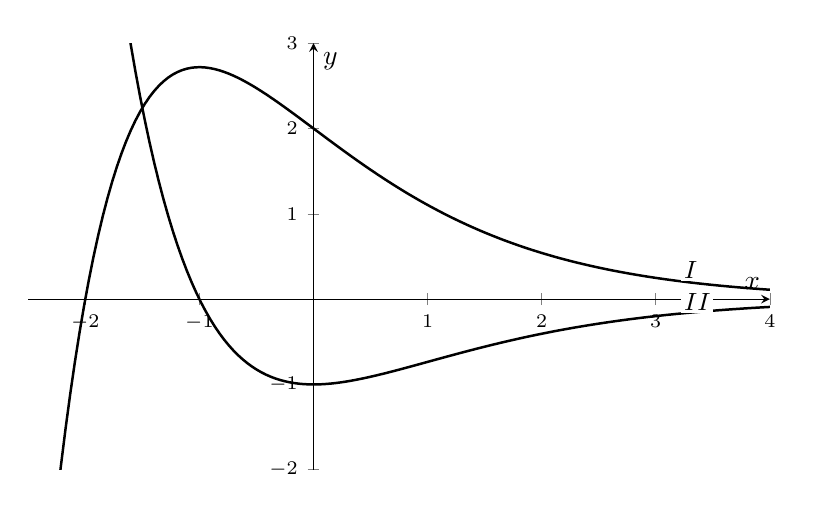
\begin{tikzpicture}\begin{axis}[xmin=-2.5,xmax=4.0,ymin=-2.0,ymax=3.0,axis lines=middle,width=11cm,height=7cm,xlabel={$x$},ylabel={$y$},tick label style={font=\scriptsize},samples=160,clip=true,every axis plot/.append style={line width=0.9pt},/pgf/number format/use comma]\addplot[black,domain=-2.5:4.0] {(x+2)*exp(-x)};\node[font=\small,fill=white,inner sep=1pt,anchor=south west] at (axis cs:3.2199999999999998,{((3.2199999999999998)+2)*exp(-(3.2199999999999998))}) {$I$};\addplot[black,domain=-2.5:4.0] {-(x+1)*exp(-x)};\node[font=\small,fill=white,inner sep=1pt,anchor=south west] at (axis cs:3.2199999999999998,{-((3.2199999999999998)+1)*exp(-(3.2199999999999998))}) {$II$};\end{axis}\end{tikzpicture}\par
\rechenplatz{1}
\fusshilfe{\mbox{46:~Graph II ist f'}}
\end{pfaufg}
\pfgruppe{}
\begin{pfaufg}{Abi ’26}{47.}{2 BE}
Die Abbildung zeigt den Schienenverlauf einer Modelleisenbahn von oben; er ist symmetrisch zur $x$-Achse und zur $y$-Achse. Für $-2 \le x \le 0$ beschreibt der Graph $G$ der Funktion $g$ mit $g(x) = \tfrac{1}{3}x^3 + x^2$ den oberen Verlauf; er beginnt in $A\left(-2 \mid \tfrac{4}{3}\right)$. Oberer und unterer Verlauf sind links und rechts durch je einen Halbkreis verbunden, der waagerecht an die Schienen anschließt. 1 LE entspricht 1 m. An der Strecke wird ein Sensor im Punkt $Q(x_Q \mid y_Q)$ mit $x_Q \neq 0$ angebracht. Für ihn gilt $y_Q = -g(-x_Q)$ und $g'(-x_Q) = 0$. Beschreibe mithilfe der Abbildung, wo der Sensor liegt.
\par\smallskip\noindent \begin{tikzpicture}\begin{axis}[xmin=-4.0,xmax=4.0,ymin=-1.5,ymax=1.5,axis lines=middle,width=11cm,xlabel={$x$},ylabel={$y$},tick label style={font=\scriptsize},samples=160,clip=true,every axis plot/.append style={line width=0.9pt},/pgf/number format/use comma,grid=both,grid style={mbgitter},minor tick num=1,axis equal image]\addplot[black,domain=-2:0] {x^3/3+x^2};\node[font=\small,fill=white,inner sep=1pt,anchor=south west] at (axis cs:-0.24,{(-0.24)^3/3+(-0.24)^2}) {$G$};\addplot[black,domain=-2:0] {-(x^3/3+x^2)};\addplot[black,domain=0:2] {-x^3/3+x^2};\addplot[black,domain=0:2] {x^3/3-x^2};\addplot[black,domain=90:270,samples=60] ({-2+1.333*cos(x)},{0+1.333*sin(x)});\addplot[black,domain=-90:90,samples=60] ({2+1.333*cos(x)},{0+1.333*sin(x)});\end{axis}\end{tikzpicture}\par
\rechenplatz{2}
\fusshilfe{\mbox{47:~Q(2 | $-\tfrac{4}{3}$)}}
\end{pfaufg}
\pfgruppe{}
\begin{pfaufg}{}{48.}{}
Der Graph einer ganzrationalen Funktion $f$ hat den Tiefpunkt $T(2 | -3)$ und keinen weiteren Extrempunkt. Beurteile ohne Rechnung: „$f'(1{,}9) > 0$“ 
\pfkreuzzeile{wahr}\pfkreuzzeile{falsch}
\end{pfaufg}
\pfgruppe{}
\begin{pfaufg}{}{49.}{}
Die Abbildung zeigt den Graphen von $f$. Gib die Nullstellen von $f'$ an und trage das Vorzeichen von $f'$ in jedem Abschnitt dazwischen ein.
\par\smallskip\noindent \begin{ksys}[xmin=-3,xmax=5,ymin=-5,ymax=5,ablesen] \funktionab{0.25*(\x-1)^3-3*(\x-1)}{f}{-3}{5} \end{ksys}\par
\rechenplatz{3}
\end{pfaufg}
\pfgruppe{}
\begin{pfaufg}{Abi ’24\\ohne Hilfsmittel}{50.}{2 BE}
Gegeben ist die in $\mathbb{R}$ definierte Funktion $f$ mit $f(x) = e^{0{,}5x} - e$; ihr Graph heißt $G$. Weise nach, dass $G$ streng monoton steigt.
\rechenplatz{2}
\fusshilfe{\mbox{50:~f'(x) = 0,5 · e$^{0{,}5x}$ > 0 für alle x}}
\end{pfaufg}
\begin{pfaufg}{Abi ’23}{51.}{3 BE}
Gegeben ist die Funktion $g$ mit $g(x) = 0{,}4x^3 - 6x^2 + 30x - 50$, $x \in \mathbb{R}$. Die Abbildung zeigt den Graphen von $g'$. Begründe mithilfe der Abbildung: (1) Der Graph von $g$ hat nur in einem Punkt eine waagerechte Tangente. (2) Der Graph von $g$ hat keinen Extrempunkt.
\par\smallskip\noindent \begin{tikzpicture}\begin{axis}[xmin=0.0,xmax=7.0,ymin=0.0,ymax=6.0,axis lines=middle,width=11cm,height=7cm,xlabel={$x$},ylabel={$y$},tick label style={font=\scriptsize},samples=160,clip=true,every axis plot/.append style={line width=0.9pt},/pgf/number format/use comma,grid=both,grid style={mbgitter},minor tick num=1]\addplot[black,domain=0.0:7.0] {1.2*(x-5)^2};\node[font=\small,fill=white,inner sep=1pt,anchor=south west] at (axis cs:6.16,{1.2*((6.16)-5)^2}) {$g'$};\end{axis}\end{tikzpicture}\par
\rechenplatz{2}
\fusshilfe{\mbox{51:~5) $\Rightarrow$ genau eine waagerechte Tangente}}
\end{pfaufg}
\pfgruppe{}
\begin{pfaufg}{Abi ’23}{52.}{2 BE}
Gegeben ist die in $\mathbb{R}$ definierte Funktion $f$ mit $f(x) = 0{,}5\cdot(x^2 - 4)\cdot e^x$; ihr Graph heißt $G$. Die erste Ableitung ist $f'(x) = (0{,}5x^2 + x - 2)\cdot e^x$. Gegeben: Der Tiefpunkt von $G$ liegt bei $x = -1 + \sqrt{5}$; für $x \ge 0$ hat $G$ keinen weiteren Extrempunkt. Gib das Monotonieverhalten von $f$ für $x \ge 0$ an.
\rechenplatz{1}
\fusshilfe{\mbox{52:~streng monoton fallend auf [0}}
\end{pfaufg}
\pfgruppe{}
\begin{pfaufg}{Abi ’23}{53.}{4 BE}
Gegeben ist die in $\mathbb{R}$ definierte Funktion $f$ mit $f(x) = 0{,}5\cdot(x^2 - 4)\cdot e^x$; ihr Graph heißt $G$. Die erste Ableitung ist $f'(x) = (0{,}5x^2 + x - 2)\cdot e^x$. Gegeben: $G$ hat genau zwei Extrempunkte, einen im II. und einen im IV. Quadranten; der Tiefpunkt ist $T(-1 + \sqrt{5} \mid f(-1 + \sqrt{5}))$. Entscheide ohne weitere Rechnung, ob die beiden Aussagen wahr sind, und begründe jeweils. (I) $f(-0{,}9 + \sqrt{5})$ ist kleiner als die $y$-Koordinate des Tiefpunkts. (II) $f'(-0{,}9 + \sqrt{5})$ ist größer als null.
\rechenplatz{2}
\fusshilfe{\mbox{53:~f'($-$0,9 + $\sqrt{5}$) > 0}}
\end{pfaufg}
\pfstufekopf[sgrenzverhaltenangebe]{Grenzverhalten angeben}{in 4 der letzten 5 Prüfungen}
\pfgruppe{Was ist zu tun? Ankreuzen, nicht rechnen}
\begin{pfaufg}{}{54.}{}
Gerade oder ungerade, plus oder minus? $f(x) = -3x^5 + x^2$
\pfkreuzzeile{Grad gerade, Koeffizient positiv}\pfkreuzzeile{Grad gerade, Koeffizient negativ}\pfkreuzzeile{Grad ungerade, Koeffizient positiv}\pfkreuzzeile{Grad ungerade, Koeffizient negativ}
\fusshilfe{\mbox{54:~Grad ungerade, Koeffizient negativ}}
\end{pfaufg}
\begin{pfaufg}{}{55.}{}
Wer gewinnt für $x \to +\infty$? $g(x) = x^2 \cdot e^{-3x}$
\pfkreuzzeile{der Faktor $x^2$}\pfkreuzzeile{der Faktor $e^{-3x}$}
\fusshilfe{\mbox{55:~der Faktor $e^{-3x}$}}
\end{pfaufg}
\pfgruppe{}
\begin{pfaufg}{}{56.}{}
$f(x) = x^2 - 6x + 1$. Verhalten für $x \to +\infty$ und $x \to -\infty$?
\par\noindent x $\to$ +∞: f(x) $\to$ \leerfeld ; x $\to$ $-$∞: f(x) $\to$ \leerfeld \par
\fusshilfe{\mbox{56:~für $x \to -\infty$: $f(x) \to +\infty$}}
\end{pfaufg}
\pfgruppe{}
\begin{pfaufg}{Abi ’22}{57.}{2 BE}
Gegeben ist die in $\mathbb{R}$ definierte Funktion $f$ mit $f(x) = (x + 2)\cdot e^{-x}$. Ihre Ableitung ist $f'(x) = -(x + 1)\cdot e^{-x}$. Gib den Grenzwert von $f(x)$ für $x \to +\infty$ an. Beschreibe, wie der Graph von $f$ für große $x$ verläuft.
\rechenplatz{1}
\fusshilfe{\mbox{57:~Grenzwert 0}}
\end{pfaufg}
\begin{pfaufg}{Abi ’22}{58.}{2 BE}
Gegeben ist die Funktion $f$ mit $f(x) = -\tfrac{1}{6}x^3 + \tfrac{1}{2}x^2$, $x \in \mathbb{R}$. Gib an, wie sich die Funktionswerte von $f$ für $x \to +\infty$ und für $x \to -\infty$ verhalten.
\rechenplatz{1}
\fusshilfe{\mbox{58:~x $\to$ +$\infty$: f(x) $\to$ $-\infty$; x $\to$ $-\infty$: f(x) $\to$ +$\infty$}}
\end{pfaufg}
\begin{pfaufg}{Abi ’26}{59.}{2 BE}
Gegeben ist die in $\mathbb{R}$ definierte Funktion $f$ mit $f(x) = \tfrac{1}{12}(x^4 + 4x^3 + 24)$. Ihre Ableitung ist $f'(x) = x^2\cdot\left(\tfrac{1}{3}x + 1\right) = \tfrac{1}{3}x^3 + x^2$; die Abbildung zeigt den Graphen von $f'$. Gib an, wie sich $f'(x)$ für $x \to -\infty$ und für $x \to +\infty$ verhält.
\par\smallskip\noindent \begin{tikzpicture}\begin{axis}[xmin=-3.0,xmax=2.0,ymin=-1.0,ymax=2.0,axis lines=middle,width=11cm,height=7cm,xlabel={$x$},ylabel={$y$},tick label style={font=\scriptsize},samples=160,clip=true,every axis plot/.append style={line width=0.9pt},/pgf/number format/use comma,grid=both,grid style={mbgitter},minor tick num=1]\addplot[black,domain=-3.0:2.0] {x^3/3+x^2};\node[font=\small,fill=white,inner sep=1pt,anchor=south west] at (axis cs:1.0,{(1.0)^3/3+(1.0)^2}) {Graph von f'};\end{axis}\end{tikzpicture}\par
\rechenplatz{1}
\fusshilfe{\mbox{59:~x $\to$ $-\infty$: f'(x) $\to$ $-\infty$; x $\to$ +$\infty$: f'(x) $\to$ +$\infty$}}
\end{pfaufg}
\begin{pfaufg}{Abi ’25}{60.}{3 BE}
Gegeben ist die Funktion $f$ mit $f(x) = (2 - x)\cdot e^x$, $x \in \mathbb{R}$; die Abbildung zeigt ihren Graphen. Gib die Nullstelle von $f$ an. Gib an, wie sich $f(x)$ für $x \to -\infty$ und für $x \to +\infty$ verhält.
\par\smallskip\noindent \begin{tikzpicture}\begin{axis}[xmin=-5.0,xmax=2.5,ymin=-0.5,ymax=3.0,axis lines=middle,width=11cm,height=7cm,xlabel={$x$},ylabel={$y$},tick label style={font=\scriptsize},samples=160,clip=true,every axis plot/.append style={line width=0.9pt},/pgf/number format/use comma,grid=both,grid style={mbgitter},minor tick num=1]\addplot[black,domain=-5.0:2.5] {(2-x)*exp(x)};\node[font=\small,fill=white,inner sep=1pt,anchor=south west] at (axis cs:1.6,{(2-(1.6))*exp((1.6))}) {$G_f$};\end{axis}\end{tikzpicture}\par
\rechenplatz{2}
\fusshilfe{\mbox{60:~Nullstelle 2; x $\to$ $-\infty$: f(x) $\to$ 0; x $\to$ +$\infty$: f(x) $\to$ $-\infty$}}
\end{pfaufg}
\pfgruppe{}
\begin{pfaufg}{Abi ’23}{61.}{2 BE}
Gegeben ist die in $\mathbb{R}$ definierte Funktion $f$ mit $f(x) = 0{,}5\cdot(x^2 - 4)\cdot e^x$; ihr Graph heißt $G$. Die erste Ableitung ist $f'(x) = (0{,}5x^2 + x - 2)\cdot e^x$. Gib an, wie sich die Funktionswerte von $f$ für $x \to +\infty$ und für $x \to -\infty$ verhalten.
\rechenplatz{1}
\fusshilfe{\mbox{61:~x $\to$ +$\infty$: f(x) $\to$ +$\infty$; x $\to$ $-\infty$: f(x) $\to$ 0}}
\end{pfaufg}
\pfstufekopf[ssymmetrieamtermbegrn]{Symmetrie am Term begründen}{in 2 der letzten 5 Prüfungen}
\pfgruppe{Was ist zu tun? Ankreuzen, nicht rechnen}
\begin{pfaufg}{}{62.}{}
$f(x) = 2x^6 - x^2 + 5$ – gerade oder ungerade Exponenten? 
\pfkreuzzeile{achsensymmetrisch}\pfkreuzzeile{punktsymmetrisch}\pfkreuzzeile{keines von beiden}
\fusshilfe{\mbox{62:~achsensymmetrisch}}
\end{pfaufg}
\pfgruppe{}
\begin{pfaufg}{}{63.}{}
Untersuche $f(x) = x^4 - 6x^2 + 1$ auf Symmetrie. Begründe am Term.
\rechenplatz{2}
\fusshilfe{\mbox{63:~prüfen: nur gerade Exponenten}}
\end{pfaufg}
\pfgruppe{}
\begin{pfaufg}{}{64.}{}
$g$ ist punktsymmetrisch zum Ursprung und hat den Tiefpunkt $T(2 | -3)$. Welcher weitere Extrempunkt folgt daraus?
\rechenplatz{2}
\end{pfaufg}
\pfgruppe{}
\begin{pfaufg}{Abi ’24\\ohne Hilfsmittel}{65.}{1 BE}
Begründe, dass der Graph der Funktion $f$ mit $f(x) = x^3 - 4x$, $x \in \mathbb{R}$, punktsymmetrisch zum Koordinatenursprung ist.
\rechenplatz{1}
\fusshilfe{\mbox{65:~nur ungerade Exponenten}}
\end{pfaufg}
\pfgruppe{}
\begin{pfaufg}{Abi ’24}{66.}{2 BE}
Gegeben ist die Funktion $f$ mit $f(x) = 0{,}5x^4 - 4x^2 + 3{,}5$, $x \in \mathbb{R}$; ihr Graph heißt $G_f$. Weise nach, dass $G_f$ achsensymmetrisch zur $y$-Achse ist.
\rechenplatz{1}
\fusshilfe{\mbox{66:~nur gerade Exponenten}}
\end{pfaufg}
\pfgruppe{}
\begin{pfaufg}{Abi ’25}{67.}{5 BE}
Gegeben ist die in $\mathbb{R}$ definierte Funktion $f$ mit $f(x) = \tfrac{2}{25}x^3 - \tfrac{3}{2}x$; ihr Graph heißt $G_f$. Aus $G_f$ und der Geraden $g$ mit $g(x) = \tfrac{1}{2}x$ wird ein Windrad gestaltet (Abbildung). Weise nach, dass $G_f$ punktsymmetrisch zum Ursprung ist. Bestimme die Nullstellen von $f$.
\par\smallskip\noindent \begin{tikzpicture}\begin{axis}[xmin=-6.0,xmax=6.0,ymin=-6.0,ymax=6.0,axis lines=middle,width=11cm,xlabel={$x$},ylabel={$y$},tick label style={font=\scriptsize},samples=160,clip=true,every axis plot/.append style={line width=0.9pt},/pgf/number format/use comma,grid=both,grid style={mbgitter},minor tick num=1,axis equal image]\addplot[black,domain=-6.0:6.0] {2/25*x^3-3/2*x};\node[font=\small,fill=white,inner sep=1pt,anchor=south west] at (axis cs:4.5600000000000005,{2/25*(4.5600000000000005)^3-3/2*(4.5600000000000005)}) {$G_f$};\addplot[black,domain=-5:5] {x/2};\node[font=\small,fill=white,inner sep=1pt,anchor=south west] at (axis cs:3.8,{(3.8)/2}) {$g$};\addplot[black!60,domain=0:360,samples=90] ({0+5.59*cos(x)},{0+5.59*sin(x)});\end{axis}\end{tikzpicture}\par
\rechenplatz{3}
\fusshilfe{\mbox{67:~$-\tfrac{2}{25}$ x³ + $\tfrac{3}{2}$ x; $\approx$ $\pm$4,33}}
\end{pfaufg}
\pfstufekopf[sgraphverschiebenspie]{Graph verschieben, spiegeln, strecken}{in 4 der letzten 5 Prüfungen}
\pfgruppe{}
\begin{pfaufg}{}{68.}{}
$f(x)$ und $f(x - 4)$ – innen oder außen? 
\pfkreuzzeile{innen: x-Richtung}\pfkreuzzeile{außen: y-Richtung}
\fusshilfe{\mbox{68:~innen: x-Richtung}}
\end{pfaufg}
\begin{pfaufg}{}{69.}{}
Gegeben ist $g(x) = f(2x + 8)$. Klammere im Argument den Faktor vor $x$ aus und gib an, um wie viel der Graph in x-Richtung verschoben ist, ohne zu zeichnen.
\par\noindent um \leerfeld[nach]  \leerfeld \par
\fusshilfe{\mbox{69:~$4$, das Plus heißt nach links}}
\end{pfaufg}
\pfgruppe{}
\begin{pfaufg}{}{70.}{}
$f(x) = x^2$ und $g(x) = (x + 2)^2$ – wie geht der Graph von $g$ aus dem von $f$ hervor?
\rechenplatz{1}
\fusshilfe{\mbox{70:~Verschiebung um $2$ nach links}}
\end{pfaufg}
\begin{pfaufg}{}{71.}{}
$f(x) = x^3$ und $g(x) = f(x) + 3$. Aussage: Beide Graphen haben an der Stelle $2$ dieselbe Steigung. Stimmt das?
\rechenplatz{2}
\fusshilfe{\mbox{71:~$12$}}
\end{pfaufg}
\pfgruppe{}
\begin{pfaufg}{}{72.}{}
$f(x) = x^3 - 12x$ hat den Hochpunkt $H(-2 | 16)$. Der Graph wird um $3$ nach rechts und um $5$ nach oben verschoben. Term und Hochpunkt des Bildes?
\rechenplatz{2}
\fusshilfe{\mbox{72:~$H'(1 | 21)$}}
\end{pfaufg}
\begin{pfaufg}{}{73.}{}
$g(x) = 4x^2 - 8x + 1$ entsteht aus $f(x) = x^2$ durch Streckung in y-Richtung und Verschiebung. Streckfaktor und Verschiebungen?
\rechenplatz{2}
\end{pfaufg}
\begin{pfaufg}{}{74.}{}
Die Gerade $y = 2x$ wird um $90 ^\circ $ gegen den Uhrzeigersinn um den Ursprung gedreht. Gleichung der Bildgeraden und Bild von $P(1 | 2)$?
\rechenplatz{2}
\fusshilfe{\mbox{74:~$P'(-2 | 1)$}}
\end{pfaufg}
\pfgruppe{}
\begin{pfaufg}{Abi ’24\\ohne Hilfsmittel}{75.}{2 BE}
Gegeben sind die in $\mathbb{R}$ definierten Funktionen $g$ mit $g(x) = 2e^x - 2$ und $h$ mit $h(x) = e^x + 1$; es gilt $g'(0) = 2$. Beurteile die Aussage: „Man kann den Graphen von $g$ so in $y$-Richtung verschieben, dass der Graph von $h$ entsteht.“
\par\smallskip\noindent \begin{tikzpicture}\begin{axis}[xmin=-3.0,xmax=2.0,ymin=-2.0,ymax=4.0,axis lines=middle,width=11cm,height=7cm,xlabel={$x$},ylabel={$y$},tick label style={font=\scriptsize},samples=160,clip=true,every axis plot/.append style={line width=0.9pt},/pgf/number format/use comma,grid=both,grid style={mbgitter},minor tick num=1]\addplot[black,domain=-3.0:2.0] {2*exp(x)-2};\node[font=\small,fill=white,inner sep=1pt,anchor=south west] at (axis cs:0.8999999999999999,{2*exp((0.8999999999999999))-2}) {Graph von g};\addplot[black,domain=-3.0:2.0] {exp(x)+1};\node[font=\small,fill=white,inner sep=1pt,anchor=south west] at (axis cs:0.7,{exp((0.7))+1}) {Graph von h};\end{axis}\end{tikzpicture}\par
\rechenplatz{1}
\fusshilfe{\mbox{75:~falsch; 1}}
\end{pfaufg}
\pfgruppe{}
\begin{pfaufg}{Abi ’26}{76.}{2 BE}
Gegeben ist die Funktion $f$ mit $f(x) = 3e^x + 1$, $x \in \mathbb{R}$; ihr Graph heißt $G_f$. Der Graph der Funktion $k$ mit $k(x) = 60e^{-\tfrac{x}{400}} + 20$ entsteht aus $G_f$ unter anderem durch eine Streckung in $y$-Richtung mit dem Faktor 20. Der Faktor $-\tfrac{1}{400}$ im Exponenten bewirkt weitere Veränderungen. Gib diese an.
\par\smallskip\noindent \begin{tikzpicture}\begin{axis}[xmin=-3.0,xmax=2.0,ymin=0.0,ymax=6.0,axis lines=middle,width=11cm,height=7cm,xlabel={$x$},ylabel={$y$},tick label style={font=\scriptsize},samples=160,clip=true,every axis plot/.append style={line width=0.9pt},/pgf/number format/use comma,grid=both,grid style={mbgitter},minor tick num=1]\addplot[black,domain=-3.0:2.0] {3*exp(x)+1};\node[font=\small,fill=white,inner sep=1pt,anchor=south west] at (axis cs:0.30000000000000027,{3*exp((0.30000000000000027))+1}) {$G_f$};\end{axis}\end{tikzpicture}\par
\rechenplatz{1}
\end{pfaufg}
\begin{pfaufg}{Abi ’23}{77.}{4 BE}
Gegeben ist die Funktion $f$ mit $f(x) = x^3 - 12x^2 + 45x - 50$, $x \in \mathbb{R}$. Man kann den Term auch als $f(x) = (x - 5)\cdot(x^2 - 7x + 10)$ schreiben. Die Funktion $h$ mit $h(x) = 4x^3 - 48x^2 + 180x + 20$ beschreibt den Temperaturverlauf eines anderen Ofens. Sie entsteht aus $f$ durch $h(x) = c\cdot(f(x) + d)$. Ermittle die Werte von $c$ und $d$. Beschreibe, wie der Graph von $h$ aus dem Graphen von $f$ entsteht.
\rechenplatz{3}
\fusshilfe{\mbox{77:~55}}
\end{pfaufg}
\pfgruppe{}
\begin{pfaufg}{Abi ’24\\ohne Hilfsmittel}{78.}{3 BE}
Gegeben ist die in $\mathbb{R}$ definierte Funktion $f$ mit $f(x) = e^{0{,}5x} - e$; ihr Graph heißt $G$. $G$ wird in Richtung der $x$-Achse so verschoben, dass er durch den Ursprung geht; so entsteht der Graph einer Funktion $h$. Ermittle eine Gleichung von $h$.
\rechenplatz{2}
\fusshilfe{\mbox{78:~h(x) = f(x + 2) = e$^{0{,}5x + 1}$ $-$ e}}
\end{pfaufg}
\begin{pfaufg}{Abi ’23}{79.}{2 BE}
Gegeben ist die in $\mathbb{R}$ definierte Funktion $f$ mit $f(x) = 0{,}5\cdot(x^2 - 4)\cdot e^x$; ihr Graph heißt $G$. Die erste Ableitung ist $f'(x) = (0{,}5x^2 + x - 2)\cdot e^x$. Die Abbildung zeigt die Draufsicht auf die Platte eines Beistelltischs (1 LE entspricht 15 cm). Die Platte ist symmetrisch zu beiden Koordinatenachsen. Ihr Rand im III. Quadranten ist der Teil von $G$ zwischen $(-2 \mid 0)$ und $(0 \mid -2)$; die Ränder in den anderen drei Quadranten sind Teile der Graphen weiterer Funktionen. Gib für zwei dieser Ränder je eine Funktionsgleichung an und nenne den Quadranten.
\par\smallskip\noindent \begin{tikzpicture}\begin{axis}[xmin=-2.5,xmax=2.5,ymin=-2.5,ymax=2.5,axis lines=middle,width=11cm,height=7cm,xlabel={$x$},ylabel={$y$},tick label style={font=\scriptsize},samples=160,clip=true,every axis plot/.append style={line width=0.9pt},/pgf/number format/use comma,grid=both,grid style={mbgitter},minor tick num=1]\addplot[black,domain=-2:0] {0.5*(x^2-4)*exp(x)};\node[font=\small,fill=white,inner sep=1pt,anchor=south west] at (axis cs:-0.24,{0.5*((-0.24)^2-4)*exp((-0.24))}) {$G$};\addplot[black,domain=0:2] {0.5*(x^2-4)*exp(-x)};\addplot[black,domain=-2:0] {-0.5*(x^2-4)*exp(x)};\addplot[black,domain=0:2] {-0.5*(x^2-4)*exp(-x)};\end{axis}\end{tikzpicture}\par
\rechenplatz{2}
\fusshilfe{\mbox{79:~$-$0,5 · (x² $-$ 4) · e$^{x}$; k(x) = $-$f($-$x)}}
\end{pfaufg}
\pfgruppe{}
\begin{pfaufg}{Abi ’25}{80.}{3 BE}
Gegeben ist die in $\mathbb{R}$ definierte Funktion $f$ mit $f(x) = \tfrac{2}{25}x^3 - \tfrac{3}{2}x$; ihr Graph heißt $G_f$. Aus $G_f$ und der Geraden $g$ mit $g(x) = \tfrac{1}{2}x$ wird ein Windrad gestaltet (Abbildung). Für das Windrad werden $G_f$ und die Strecke von $g$ für $-5 \le x \le 5$ um 90° gegen den Uhrzeigersinn um den Ursprung gedreht. Dabei wird $g$ zur Geraden $g^*$ und der Punkt $A(5 \mid 2{,}5)$, in dem sich $G_f$ und $g$ schneiden, zum Punkt $A^*$. Begründe, dass $g^*(x) = -2x$ gilt. Gib die Koordinaten von $A^*$ an.
\par\smallskip\noindent \begin{tikzpicture}\begin{axis}[xmin=-6.0,xmax=6.0,ymin=-6.0,ymax=6.0,axis lines=middle,width=11cm,xlabel={$x$},ylabel={$y$},tick label style={font=\scriptsize},samples=160,clip=true,every axis plot/.append style={line width=0.9pt},/pgf/number format/use comma,grid=both,grid style={mbgitter},minor tick num=1,axis equal image]\addplot[black,domain=-6.0:6.0] {2/25*x^3-3/2*x};\node[font=\small,fill=white,inner sep=1pt,anchor=south west] at (axis cs:4.5600000000000005,{2/25*(4.5600000000000005)^3-3/2*(4.5600000000000005)}) {$G_f$};\addplot[black,domain=-5:5] {x/2};\node[font=\small,fill=white,inner sep=1pt,anchor=south west] at (axis cs:3.8,{(3.8)/2}) {$g$};\addplot[black!60,domain=0:360,samples=90] ({0+5.59*cos(x)},{0+5.59*sin(x)});\end{axis}\end{tikzpicture}\par
\rechenplatz{2}
\fusshilfe{\mbox{80:~$-$2x; A*($-$2,5 | 5)}}
\end{pfaufg}
\pfgruppe{}
\begin{pfaufg}{Abi ’26\\ohne Hilfsmittel}{81.}{3 BE}
Gegeben ist die in $\mathbb{R}$ definierte Funktion $f$ mit $f(x) = \sin x$. Drei direkt aufeinanderfolgende Extrempunkte ihres Graphen, $A\left(\tfrac{\pi}{2} \mid 1\right)$, $B\left(\tfrac{3\pi}{2} \mid -1\right)$ und $C\left(\tfrac{5\pi}{2} \mid 1\right)$, sind die Ecken des Dreiecks $ABC$ (Abbildung). Gegeben ist die Funktion $g$ mit $g(x) = 2\cdot\sin\left(\tfrac{1}{3}x\right)$, $x \in \mathbb{R}$. Betrachte die Strecke zwischen zwei direkt aufeinanderfolgenden Extrempunkten des Graphen von $g$. Untersuche, ob diese Strecke kürzer ist als die Strecke $AB$.
\par\smallskip\noindent \begin{tikzpicture}\begin{axis}[xmin=0.0,xmax=9.43,ymin=-1.5,ymax=1.5,axis lines=middle,width=11cm,height=7cm,xlabel={$x$},ylabel={$y$},tick label style={font=\scriptsize},samples=160,clip=true,every axis plot/.append style={line width=0.9pt},/pgf/number format/use comma,xtick={1.5708,3.1416,4.7124,6.2832,7.854,9.4248},xticklabels={$\frac{\pi}{2}$,$\pi$,$\frac{3\pi}{2}$,$2\pi$,$\frac{5\pi}{2}$,$3\pi$}]\addplot[black,dashed,domain=0.0:9.43] {sin(deg(x))};\node[font=\small,fill=white,inner sep=1pt,anchor=south west] at (axis cs:8.298399999999999,{sin(deg((8.298399999999999)))}) {$sin$};\draw[black] (axis cs:1.571,1) -- (axis cs:4.712,-1) -- (axis cs:7.854,1) -- (axis cs:1.571,1);\end{axis}\end{tikzpicture}\par
\rechenplatz{2}
\fusshilfe{\mbox{81:~nein}}
\end{pfaufg}
\pfgruppe{}
\begin{pfaufg}{Abi ’26}{82.}{4 BE}
Gegeben ist die Gerade $t$ mit $t(x) = \tfrac{4}{3}x + \tfrac{10}{3}$. Verschiebt man $t$ um $z$ Einheiten in negative $y$-Richtung, entsteht eine Gerade $h$, die von $t$ den Abstand 5 hat. Ermittle einen Wert für $z$; die Abbildung hilft dir dabei.
\par\smallskip\noindent \fbox{\parbox{0.9\linewidth}{\footnotesize Skizze: Koordinatensystem ohne Skalierung mit den parallelen Geraden t (durch ihren y-Achsenabschnitt) und h darunter; Lot vom y-Achsenabschnitt von t auf h mit rechtem Winkel; Beschriftungen t, h}}\par
\rechenplatz{3}
\fusshilfe{\mbox{82:~z = $\tfrac{25}{3}$ $\approx$ 8,33}}
\end{pfaufg}
\pfgruppe{}
\begin{pfaufg}{Abi ’24}{83.}{3 BE}
Gegeben ist die in $\mathbb{R}$ definierte Funktion $f$ mit $f(x) = (x - 2)\cdot e^{-\tfrac{x}{2} + 3}$ und ihrer Ableitung $f'(x) = \left(-\tfrac{x}{2} + 2\right)\cdot e^{-\tfrac{x}{2} + 3}$. Die Abbildung zeigt den Graphen $G_f$ und den Graphen von $f'$. Ein Schrankknauf entsteht, wenn $G_f$ für $2 \le x \le 11$ um die $x$-Achse rotiert. Die Abbildung zeigt seinen Querschnitt: oben begrenzt durch $G_f$, unten durch den Graphen einer Funktion $g$, der durch Spiegelung von $G_f$ an der $x$-Achse entsteht. Der Sockel liegt bei $x = 11$; 1 LE entspricht 0,5 cm. Gib eine Gleichung von $g$ an. Bestimme den Durchmesser des Sockels in Millimetern.
\par\smallskip\noindent \begin{tikzpicture}\begin{axis}[xmin=0.0,xmax=12.0,ymin=-6.0,ymax=6.0,axis lines=middle,width=11cm,height=7cm,xlabel={$x$},ylabel={$y$},tick label style={font=\scriptsize},samples=160,clip=true,every axis plot/.append style={line width=0.9pt},/pgf/number format/use comma]\addplot[black,domain=2:11] {(x-2)*exp(-x/2+3)};\node[font=\small,fill=white,inner sep=1pt,anchor=south west] at (axis cs:9.92,{((9.92)-2)*exp(-(9.92)/2+3)}) {$G_f$};\addplot[black,domain=2:11] {-(x-2)*exp(-x/2+3)};\node[font=\small,fill=white,inner sep=1pt,anchor=south west] at (axis cs:9.92,{-((9.92)-2)*exp(-(9.92)/2+3)}) {$G_g$};\draw[black] (axis cs:11,-0.739) -- (axis cs:11,0.739);\end{axis}\end{tikzpicture}\par
\rechenplatz{3}
\fusshilfe{\mbox{83:~g(x) = $-$(x $-$ 2) · e$^{-x/2 + 3}$; $\approx$ 7,4 mm}}
\end{pfaufg}
\pfstufekopf[smaeimsachzusammenhan]{Maße im Sachzusammenhang aus dem Graphen berechnen}{in 4 der letzten 5 Prüfungen}
\pfgruppe{}
\begin{pfaufg}{}{84.}{}
$f(x) = x^2 + 1$ und $g(x) = 2x - 3$ – senkrechter Abstand der Graphenpunkte an der Stelle $3$?
\rechenplatz{2}
\fusshilfe{\mbox{84:~$7$}}
\end{pfaufg}
\pfgruppe{}
\begin{pfaufg}{}{85.}{}
Ein Spielball ist rotationssymmetrisch, sein Rand wird durch $f(x) = -\tfrac{1}{8}x^2 + 2$ beschrieben (1 Längeneinheit entspricht 5 cm, Achse auf der x-Achse). Länge des Balls?
\rechenplatz{3}
\fusshilfe{\mbox{85:~$40$ cm}}
\end{pfaufg}
\begin{pfaufg}{Abi ’26\\ohne Hilfsmittel}{86.}{2 BE}
Gegeben ist die in $\mathbb{R}$ definierte Funktion $f$ mit $f(x) = \sin x$. Drei direkt aufeinanderfolgende Extrempunkte ihres Graphen, $A\left(\tfrac{\pi}{2} \mid 1\right)$, $B\left(\tfrac{3\pi}{2} \mid -1\right)$ und $C\left(\tfrac{5\pi}{2} \mid 1\right)$, sind die Ecken des Dreiecks $ABC$ (Abbildung). Berechne den Flächeninhalt des Dreiecks $ABC$.
\par\smallskip\noindent \begin{tikzpicture}\begin{axis}[xmin=0.0,xmax=9.43,ymin=-1.5,ymax=1.5,axis lines=middle,width=11cm,height=7cm,xlabel={$x$},ylabel={$y$},tick label style={font=\scriptsize},samples=160,clip=true,every axis plot/.append style={line width=0.9pt},/pgf/number format/use comma,xtick={1.5708,3.1416,4.7124,6.2832,7.854,9.4248},xticklabels={$\frac{\pi}{2}$,$\pi$,$\frac{3\pi}{2}$,$2\pi$,$\frac{5\pi}{2}$,$3\pi$}]\addplot[black,dashed,domain=0.0:9.43] {sin(deg(x))};\node[font=\small,fill=white,inner sep=1pt,anchor=south west] at (axis cs:8.298399999999999,{sin(deg((8.298399999999999)))}) {$sin$};\draw[black] (axis cs:1.571,1) -- (axis cs:4.712,-1) -- (axis cs:7.854,1) -- (axis cs:1.571,1);\end{axis}\end{tikzpicture}\par
\rechenplatz{2}
\fusshilfe{\mbox{86:~A = $\tfrac{1}{2}$ · 2$\pi$ · 2 = 2$\pi$}}
\end{pfaufg}
\pfgruppe{}
\begin{pfaufg}{}{87.}{}
Ein Brückenbogen wird durch $f(x) = -0{,}1x^2 + 2{,}5$ beschrieben, oberhalb der $x$-Achse (1 LE = 2 m). Wie breit und wie hoch ist der Bogen in Metern?
\rechenplatz{3}
\fusshilfe{\mbox{87:~$5$ m}}
\end{pfaufg}
\begin{pfaufg}{Abi ’23}{88.}{4 BE}
Gegeben ist die in $\mathbb{R}$ definierte Funktion $f$ mit $f(x) = 0{,}5\cdot(x^2 - 4)\cdot e^x$; ihr Graph heißt $G$. Die erste Ableitung ist $f'(x) = (0{,}5x^2 + x - 2)\cdot e^x$. Gegeben: Die Spitzen der Tischplatte liegen bei $(\pm 2 \mid 0)$ und $(0 \mid \pm 2)$; 1 LE entspricht 15 cm. Der Tisch ist 0,5 m hoch und wird in einem quaderförmigen Karton mit quadratischer Grundfläche geliefert. Die Kanten der Grundfläche verlaufen parallel zu den Koordinatenachsen. Bestimme, wie viele Liter der Karton mindestens fassen muss.
\rechenplatz{3}
\fusshilfe{\mbox{88:~180 l}}
\end{pfaufg}
\pfgruppe{}
\begin{pfaufg}{Abi ’26}{89.}{2 BE}
Die Abbildung zeigt den Schienenverlauf einer Modelleisenbahn von oben; er ist symmetrisch zur $x$-Achse und zur $y$-Achse. Für $-2 \le x \le 0$ beschreibt der Graph $G$ der Funktion $g$ mit $g(x) = \tfrac{1}{3}x^3 + x^2$ den oberen Verlauf; er beginnt in $A\left(-2 \mid \tfrac{4}{3}\right)$. Oberer und unterer Verlauf sind links und rechts durch je einen Halbkreis verbunden, der waagerecht an die Schienen anschließt. 1 LE entspricht 1 m. Weise nach, dass der ganze Schienenverlauf auf eine rechteckige Holzplatte von 2,7 m mal 6,7 m passt.
\par\smallskip\noindent \begin{tikzpicture}\begin{axis}[xmin=-4.0,xmax=4.0,ymin=-1.5,ymax=1.5,axis lines=middle,width=11cm,xlabel={$x$},ylabel={$y$},tick label style={font=\scriptsize},samples=160,clip=true,every axis plot/.append style={line width=0.9pt},/pgf/number format/use comma,grid=both,grid style={mbgitter},minor tick num=1,axis equal image]\addplot[black,domain=-2:0] {x^3/3+x^2};\node[font=\small,fill=white,inner sep=1pt,anchor=south west] at (axis cs:-0.24,{(-0.24)^3/3+(-0.24)^2}) {$G$};\addplot[black,domain=-2:0] {-(x^3/3+x^2)};\addplot[black,domain=0:2] {-x^3/3+x^2};\addplot[black,domain=0:2] {x^3/3-x^2};\addplot[black,domain=90:270,samples=60] ({-2+1.333*cos(x)},{0+1.333*sin(x)});\addplot[black,domain=-90:90,samples=60] ({2+1.333*cos(x)},{0+1.333*sin(x)});\end{axis}\end{tikzpicture}\par
\rechenplatz{2}
\fusshilfe{\mbox{89:~passt; $\tfrac{20}{3}$ m $\approx$ 6,67 m $\le$ 6,7 m}}
\end{pfaufg}
\pfgruppe{}
\begin{pfaufg}{Abi ’22}{90.}{3 BE}
Ein Tauchroboter bewegt sich 30 Minuten lang nur senkrecht nach unten und oben. Sein Abstand von der Wasseroberfläche wird beschrieben durch $h(t) = \tfrac{9}{40}t^3 - \tfrac{27}{2}t^2 + \tfrac{405}{2}t$ mit $0 \le t \le 30$ ($t$: Zeit in Minuten, $h(t)$: Abstand in Metern). Gegeben: Den größten Abstand von 900 m erreicht der Roboter nach 10 Minuten. Berechne den Weg, den er in den ersten 15 Minuten insgesamt zurücklegt.
\par\smallskip\noindent \begin{tikzpicture}\begin{axis}[xmin=0.0,xmax=30.0,ymin=0.0,ymax=1000.0,axis lines=middle,width=11cm,height=7cm,xlabel={$t$},ylabel={$h(t)$},tick label style={font=\scriptsize},samples=160,clip=true,every axis plot/.append style={line width=0.9pt},/pgf/number format/use comma,grid=both,grid style={mbgitter},minor tick num=1]\addplot[black,domain=0.0:30.0] {9/40*x^3-27/2*x^2+405/2*x};\node[font=\small,fill=white,inner sep=1pt,anchor=south west] at (axis cs:25.8,{9/40*(25.8)^3-27/2*(25.8)^2+405/2*(25.8)}) {$G_h$};\end{axis}\end{tikzpicture}\par
\rechenplatz{2}
\fusshilfe{\mbox{90:~$\approx$ 1041 m}}
\end{pfaufg}
\begin{pfaufg}{Abi ’26}{91.}{3 BE}
Die Abbildung zeigt den Schienenverlauf einer Modelleisenbahn von oben; er ist symmetrisch zur $x$-Achse und zur $y$-Achse. Für $-2 \le x \le 0$ beschreibt der Graph $G$ der Funktion $g$ mit $g(x) = \tfrac{1}{3}x^3 + x^2$ den oberen Verlauf; er beginnt in $A\left(-2 \mid \tfrac{4}{3}\right)$. Oberer und unterer Verlauf sind links und rechts durch je einen Halbkreis verbunden, der waagerecht an die Schienen anschließt. 1 LE entspricht 1 m. Der Bogen des Schienenverlaufs von $A$ bis zum Ursprung ist etwa 2,5 m lang. Ein Zug fährt 3,5 m pro Minute. Ermittle, wie lange er für eine ganze Runde braucht.
\par\smallskip\noindent \begin{tikzpicture}\begin{axis}[xmin=-4.0,xmax=4.0,ymin=-1.5,ymax=1.5,axis lines=middle,width=11cm,xlabel={$x$},ylabel={$y$},tick label style={font=\scriptsize},samples=160,clip=true,every axis plot/.append style={line width=0.9pt},/pgf/number format/use comma,grid=both,grid style={mbgitter},minor tick num=1,axis equal image]\addplot[black,domain=-2:0] {x^3/3+x^2};\node[font=\small,fill=white,inner sep=1pt,anchor=south west] at (axis cs:-0.24,{(-0.24)^3/3+(-0.24)^2}) {$G$};\addplot[black,domain=-2:0] {-(x^3/3+x^2)};\addplot[black,domain=0:2] {-x^3/3+x^2};\addplot[black,domain=0:2] {x^3/3-x^2};\addplot[black,domain=90:270,samples=60] ({-2+1.333*cos(x)},{0+1.333*sin(x)});\addplot[black,domain=-90:90,samples=60] ({2+1.333*cos(x)},{0+1.333*sin(x)});\end{axis}\end{tikzpicture}\par
\rechenplatz{3}
\fusshilfe{\mbox{91:~Länge $\approx$ 18,4 m; Zeit $\approx$ 5,25 min $\approx$ 5 min 15 s}}
\end{pfaufg}
\pfgruppe{}
\begin{pfaufg}{Abi ’24}{92.}{4 BE}
Gegeben ist die in $\mathbb{R}$ definierte Funktion $f$ mit $f(x) = (x - 2)\cdot e^{-\tfrac{x}{2} + 3}$ und ihrer Ableitung $f'(x) = \left(-\tfrac{x}{2} + 2\right)\cdot e^{-\tfrac{x}{2} + 3}$. Die Abbildung zeigt den Graphen $G_f$ und den Graphen von $f'$. Gegeben: Der Hochpunkt von $G_f$ ist $(4 \mid 2e)$. Der Schrankknauf (Rotationskörper von $G_f$ um die $x$-Achse für $2 \le x \le 11$, 1 LE entspricht 0,5 cm) wird aus einem quaderförmigen Holzstück gedreht; das Holz hat die Dichte 0,86 g/cm³. Gib die Maße an, die das Holzstück mindestens haben muss. Berechne die Masse dieses Holzstücks.
\par\smallskip\noindent \begin{tikzpicture}\begin{axis}[xmin=0.0,xmax=12.0,ymin=-3.0,ymax=7.0,axis lines=middle,width=11cm,height=7cm,xlabel={$x$},ylabel={$y$},tick label style={font=\scriptsize},samples=160,clip=true,every axis plot/.append style={line width=0.9pt},/pgf/number format/use comma]\addplot[black,domain=0.0:12.0] {(x-2)*exp(-x/2+3)};\node[font=\small,fill=white,inner sep=1pt,anchor=south west] at (axis cs:10.56,{((10.56)-2)*exp(-(10.56)/2+3)}) {$G_f$};\addplot[black,dashed,domain=0.0:12.0] {(-x/2+2)*exp(-x/2+3)};\node[font=\small,fill=white,inner sep=1pt,anchor=south west] at (axis cs:10.56,{(-(10.56)/2+2)*exp(-(10.56)/2+3)}) {$f'$};\end{axis}\end{tikzpicture}\par
\rechenplatz{4}
\fusshilfe{\mbox{92:~4,5 cm $\times$ 5,44 cm $\times$ 5,44 cm; Masse $\approx$ 114 g}}
\end{pfaufg}
\pfstufekopf[sgleichungenundunglei]{Gleichungen und Ungleichungen zwischen Funktionen lösen}{in 4 der letzten 5 Prüfungen}
\pfgruppe{Was ist zu tun? Ankreuzen, nicht rechnen}
\begin{pfaufg}{}{93.}{}
Welcher Weg? $x^4 - 10x^2 + 9 = 0$
\pfkreuzzeile{Lösungsformel}\pfkreuzzeile{Substitution}\pfkreuzzeile{Polynomdivision}
\fusshilfe{\mbox{93:~Substitution}}
\end{pfaufg}
\begin{pfaufg}{}{94.}{}
Welche Lösungen zählen? $x^2 \cdot (x - 3) > 0$
\pfkreuzzeile{$x > 3$}\pfkreuzzeile{$x > 3$ und $x = 0$}\pfkreuzzeile{$x \ge 3$}
\fusshilfe{\mbox{94:~$x > 3$}}
\end{pfaufg}
\pfgruppe{}
\begin{pfaufg}{}{95.}{}
$f(x) = x^2 - 2x - 1$, $g(x) = x + 9$. Schnittpunkte?
\par\noindent S1( \leerfeld[|]  \leerfeld[)] , S2( \leerfeld[|]  \leerfeld[)] \par
\fusshilfe{\mbox{95:~$S_1(-2 | 7)$, $S_2(5 | 14)$}}
\end{pfaufg}
\begin{pfaufg}{}{96.}{}
Für welche $x$ gilt $(x - 1) \cdot (x + 2)^2 > 0$?
\par\noindent \leerfeld \par
\fusshilfe{\mbox{96:~$x > 1$}}
\end{pfaufg}
\pfgruppe{}
\begin{pfaufg}{}{97.}{}
Der Graph zeigt die Höhe $h(t)$ einer Drohne ($t$ in s, $h$ in m). Wann ist sie 4 m hoch? Schreibe die Gleichung und lies ab.
\par\smallskip\noindent \begin{ksys}[xmin=0,xmax=6,ymin=0,ymax=6,ablesen] \parabel{-1}{3}{5}{h} \end{ksys}\par
\par\noindent Gleichung: \leerfeld , t = \leerfeld \par
\fusshilfe{\mbox{97:~$t_1 = 2$, $t_2 = 4$}}
\end{pfaufg}
\pfgruppe{}
\begin{pfaufg}{nach Abi ’23}{98.}{5 BE}
$f(x) = -x^3 + 5x^2 - 10x + 2$, $g(x) = -3x^2 + 6x + 2$. Bestimme rechnerisch alle $x$ mit $f(x) > g(x)$.
\par\noindent \leerfeld \par
\fusshilfe{\mbox{98:~$4$ ist die Differenz null: $x < 0$}}
\end{pfaufg}
\pfgruppe{}
\begin{pfaufg}{nach Abi ’25}{99.}{5 BE}
$a(x)$ ist die Zahl der Abonnenten eines Kanals in Hundert, $x$ in Wochen (Graph). Löse $a(x + 2) = a(x) + 6$ grafisch und deute die Lösung.
\par\smallskip\noindent \begin{ksys}[xmin=0,xmax=6,ymin=0,ymax=10,ablesen] \parabel{0.5}{0}{0}{a} \end{ksys}\par
\par\noindent x = \leerfeld \par
\fusshilfe{\mbox{99:~$2$}}
\end{pfaufg}
\pfgruppe{}
\begin{pfaufg}{nach Abi ’25}{100.}{3 BE}
$f(x) = -x^2 + 6x - 4$. Bilde $f'(x)$ und löse $\tfrac{f(x) - 0}{x - 0} = f'(x)$ rechnerisch.
\par\noindent f'(x) = \leerfeld , x1 = \leerfeld , x2 = \leerfeld \par
\fusshilfe{\mbox{100:~$x_1 = 2$, $x_2 = -2$}}
\end{pfaufg}
\pfgruppe{}
\begin{pfaufg}{Abi ’25\\ohne Hilfsmittel}{101.}{3 BE}
Gegeben ist die in $\mathbb{R}$ definierte Funktion $f$ mit $f(x) = -x^2 + 4x - 1$; die Abbildung zeigt ihren Graphen. Gib einen Term von $f'$ an. Ermittle rechnerisch alle Lösungen der Gleichung $\tfrac{f(x) - 0}{x - 0} = f'(x)$.
\par\smallskip\noindent \begin{tikzpicture}\begin{axis}[xmin=-2.0,xmax=6.0,ymin=-6.0,ymax=3.0,axis lines=middle,width=11cm,height=7cm,xlabel={$x$},ylabel={$y$},tick label style={font=\scriptsize},samples=160,clip=true,every axis plot/.append style={line width=0.9pt},/pgf/number format/use comma,grid=both,grid style={mbgitter},minor tick num=1]\addplot[black,domain=-2.0:6.0] {-x^2+4*x-1};\node[font=\small,fill=white,inner sep=1pt,anchor=south west] at (axis cs:4.72,{-(4.72)^2+4*(4.72)-1}) {$G_f$};\end{axis}\end{tikzpicture}\par
\rechenplatz{3}
\fusshilfe{\mbox{101:~f'(x) = $-$2x + 4; x = $-$1 oder x = 1}}
\end{pfaufg}
\pfgruppe{}
\begin{pfaufg}{Abi ’22}{102.}{2 BE}
Gegeben ist die in $\mathbb{R}$ definierte Funktion $f$ mit $f(x) = (x + 2)\cdot e^{-x}$. Ihre Ableitung ist $f'(x) = -(x + 1)\cdot e^{-x}$. Weise nach, dass sich die Graphen von $f$ und $f'$ an der Stelle $x = -1{,}5$ schneiden.
\rechenplatz{2}
\fusshilfe{\mbox{102:~$-$1,5}}
\end{pfaufg}
\pfgruppe{}
\begin{pfaufg}{Abi ’23}{103.}{5 BE}
Gegeben ist die Funktion $f$ mit $f(x) = x^3 - 12x^2 + 45x - 50$, $x \in \mathbb{R}$. Man kann den Term auch als $f(x) = (x - 5)\cdot(x^2 - 7x + 10)$ schreiben. Gegeben ist außerdem $g(x) = 0{,}4x^3 - 6x^2 + 30x - 50$. Bestimme rechnerisch alle $x \in \mathbb{R}$, für die $f(x) > g(x)$ gilt.
\rechenplatz{4}
\fusshilfe{\mbox{103:~L = (0; 5) $\cup$ (5; $\infty$)}}
\end{pfaufg}
\pfgruppe{}
\begin{pfaufg}{Abi ’24}{104.}{3 BE}
Gegeben ist die Funktion $f$ mit $f(x) = 0{,}5x^4 - 4x^2 + 3{,}5$, $x \in \mathbb{R}$; ihr Graph heißt $G_f$. Gegeben: Für $-1 \le x \le 1$ beträgt die größte Differenz von $p(x) = -3{,}5x^2 + 3{,}5$ und $f(x)$ genau $\tfrac{1}{8}$. Für $x \ge 1$ soll $p$ als Näherung für $f$ gelten, solange der Betrag der Differenz höchstens dreimal so groß ist wie diese größte Differenz. Beschreibe einen Lösungsweg, mit dem du alle $x \ge 1$ ermittelst, für die $p$ als Näherung geeignet ist.
\rechenplatz{3}
\fusshilfe{\mbox{104:~$\approx$ 1,22}}
\end{pfaufg}
\pfgruppe{}
\begin{pfaufg}{Abi ’25}{105.}{5 BE}
Unter einem Beitrag auf einer Internetseite werden Likes gesammelt. $a(x)$ ist die Anzahl der Likes, die seit 12:00 Uhr abgegeben wurden; $x$ ist die Zeit in Stunden seit 12:00 Uhr. Die Abbildung zeigt den Graphen von $a$. Die Gleichung $a(x + 3) = a(x) + 1000$ hat für $x > 0$ genau eine Lösung. Ermittle diese Lösung grafisch mithilfe der Abbildung. Deute die Gleichung im Sachzusammenhang.
\par\smallskip\noindent \fbox{\parbox{0.9\linewidth}{\footnotesize Skizze: x von 0 bis 7 (Stunden), y von 0 bis 3000; Graph steigt von 0 erst immer steiler, ab etwa x = 1 immer flacher und nähert sich 2500; a(2) $\approx$ 1500, a(4) $\approx$ 2300}}\par
\rechenplatz{3}
\fusshilfe{\mbox{105:~$\approx$ 1,9}}
\end{pfaufg}
\pfstufekopf[sgraphskizzierenundve]{Graph skizzieren und Verlauf beschreiben}{in 2 der letzten 5 Prüfungen}
\pfgruppe{Was ist zu tun? Ankreuzen, nicht rechnen}
\begin{pfaufg}{}{106.}{}
$f(x) = -2x^4 + x$ – wohin verläuft der Graph für $x \to +\infty$? 
\pfkreuzzeile{nach oben}\pfkreuzzeile{nach unten}
\fusshilfe{\mbox{106:~nach unten}}
\end{pfaufg}
\begin{pfaufg}{}{107.}{}
$f(x) = x^3 - 5x + 2$ – wo schneidet der Graph die y-Achse? 
\pfkreuzzeile{$(0 | 2)$}\pfkreuzzeile{$(0 | -5)$}\pfkreuzzeile{$(0 | 0)$}
\fusshilfe{\mbox{107:~$(0 | 2)$}}
\end{pfaufg}
\pfgruppe{}
\begin{pfaufg}{}{108.}{}
Fülle die Wertetabelle von $f(x) = x^3 - x$ aus und übertrage die Punkte ins Koordinatensystem.
\par\smallskip\noindent \wertetabelle{x}{f(x)}{-2,-1,0,1,2}\begin{ksys}[xmin=-3,xmax=3,ymin=-7,ymax=7]\end{ksys}\par
\end{pfaufg}
\pfgruppe{}
\begin{pfaufg}{Abi ’25}{109.}{2 BE}
Unter einem Beitrag auf einer Internetseite werden Likes gesammelt. $a(x)$ ist die Anzahl der Likes, die seit 12:00 Uhr abgegeben wurden; $x$ ist die Zeit in Stunden seit 12:00 Uhr. Die Abbildung zeigt den Graphen von $a$. Beschreibe den Verlauf des Graphen von $a$ im Sachzusammenhang.
\par\smallskip\noindent \fbox{\parbox{0.9\linewidth}{\footnotesize Skizze: x von 0 bis 7 (Stunden), y von 0 bis 3000; Graph steigt von 0 erst immer steiler, ab etwa x = 1 immer flacher und nähert sich 2500; a(2) $\approx$ 1500, a(4) $\approx$ 2300}}\par
\rechenplatz{1}
\end{pfaufg}
\pfgruppe{}
\begin{pfaufg}{}{110.}{}
$f(x) = 0{,}5x^4 - 4x^2$ hat die Tiefpunkte $(-2 | -8)$ und $(2 | -8)$ und den Hochpunkt im Ursprung. Berechne die Randwerte und zeichne den Graphen für $-3 \le x \le 3$.
\par\smallskip\noindent \begin{ksys}[xmin=-4,xmax=4,ymin=-9,ymax=5]\end{ksys}\par
\rechenplatz{2}
\fusshilfe{\mbox{110:~$4{,}5$}}
\end{pfaufg}
\pfgruppe{}
\begin{pfaufg}{Abi ’23}{111.}{1 BE}
Ein Hersteller prüft Temperatursteuerungen für Backöfen. Nach dem Einschalten steigt die Temperatur; ist die Solltemperatur erreicht, schaltet die Heizung ab, und unter einem bestimmten Wert schaltet sie wieder ein. Die Abbildung zeigt den Temperaturverlauf. Die ersten 5 Minuten heißen Startphase, die Zeit danach Dauerphase. Gib näherungsweise die durchschnittliche Temperatur in der Dauerphase an.
\par\smallskip\noindent \fbox{\parbox{0.9\linewidth}{\footnotesize Skizze: Gitter, Zeit in Minuten von 0 bis 20 (beschriftet 2, 4, …, 18), Temperatur in °C von 20 bis 260 in Schritten von 20; Kurve von (0 | 20) steil ansteigend, bei etwa 2 min 200 °C, Maximum etwa 238 °C bei 3,5 min, danach wellenförmig mit Tiefs bei etwa 222 °C (5,5; 9,5; 13,5; 17,5 min) und Hochs bei etwa 240 bis 245 °C (7,5; 11,5; 15,5; 19,5 min)}}\par
\rechenplatz{1}
\fusshilfe{\mbox{111:~$\approx$ 230 °C (228 bis 235 °C vertretbar)}}
\end{pfaufg}
\pfgruppe{}
\begin{pfaufg}{Abi ’23}{112.}{4 BE}
Gegeben ist die Funktion $f$ mit $f(x) = x^3 - 12x^2 + 45x - 50$, $x \in \mathbb{R}$. Man kann den Term auch als $f(x) = (x - 5)\cdot(x^2 - 7x + 10)$ schreiben. Gegeben: Der Graph von $f$ hat den Hochpunkt $H(3 \mid 4)$, den Tiefpunkt $T(5 \mid 0)$ und den Wendepunkt $W(4 \mid 2)$. Skizziere den Graphen von $f$ für $0 \le x \le 7$. Beurteile mithilfe deiner Skizze die Aussage: „Jede Tangente an den Graphen von $f$ hat mit dem Graphen zwei gemeinsame Punkte.“
\rechenplatz{3}
\fusshilfe{\mbox{112:~falsch}}
\end{pfaufg}
\pfstufekopf[sfunktionsgleichungau]{Funktionsgleichung aus Bedingungen aufstellen}{in 2 der letzten 5 Prüfungen}
\pfgruppe{Was ist zu tun? Ankreuzen, nicht rechnen}
\begin{pfaufg}{}{113.}{}
„Der Graph von $f$ hat den Hochpunkt $H(3|1)$.“ Wie viele Gleichungen stecken in diesem Satz? 
\pfkreuzzeile{eine Gleichung}\pfkreuzzeile{zwei Gleichungen}
\fusshilfe{\mbox{113:~$f(3) = 1$ und $f'(3) = 0$}}
\end{pfaufg}
\begin{pfaufg}{}{114.}{}
Gesucht ist eine quadratische Funktion $f(x) = ax^2 + bx + c$; bekannt sind drei Punkte des Graphen. Reichen die Angaben? 
\pfkreuzzeile{zu wenig}\pfkreuzzeile{genau passend}\pfkreuzzeile{mehr als nötig}
\fusshilfe{\mbox{114:~drei Unbekannte $a$, $b$, $c$ und drei Gleichungen}}
\end{pfaufg}
\pfgruppe{}
\begin{pfaufg}{}{115.}{}
Bestimme die Gleichung der Geraden durch $A(1|5)$ und $B(4|14)$.
\par\noindent y = \leerfeld \par
\fusshilfe{\mbox{115:~$3x + 2$}}
\end{pfaufg}
\pfgruppe{}
\begin{pfaufg}{}{116.}{}
Der Graph einer quadratischen Funktion $f$ verläuft durch $A(0|-1)$ und hat den Tiefpunkt $T(1|-3)$. Bestimme eine Funktionsgleichung von $f$.
\par\noindent f(x) = \leerfeld \par
\fusshilfe{\mbox{116:~$2x^2 - 4x - 1$}}
\end{pfaufg}
\pfgruppe{}
\begin{pfaufg}{nach Abi ’22}{117.}{2 BE}
Die Gerade $h$ verläuft durch $C(0{,}6|1{,}2)$ und $D(3|6)$. Weise nach, dass $h(x) = 2x$ eine Gleichung von $h$ ist.
\rechenplatz{2}
\end{pfaufg}
\pfgruppe{}
\begin{pfaufg}{Abi ’22}{118.}{2 BE}
Ein Betonteil für den Hochwasserschutz hat im Querschnitt einen geraden unteren Rand. Er liegt auf der Geraden $g$ durch $C(0{,}4 \mid -0{,}4)$ und $D(2 \mid 1{,}2)$. Weise nach, dass $g(x) = x - 0{,}8$ eine Gleichung dieser Geraden ist.
\par\smallskip\noindent \fbox{\parbox{0.9\linewidth}{\footnotesize Skizze: Querschnitt eines Betonteils: oberer Rand von A (Ursprung) nach B(2 | 1,5) als s-förmiger Bogen, unterer Rand Gerade von C(0,4 | $-$0,4) nach D(2 | 1,2), Seiten AC und BD; Beschriftungen A, B, C, D}}\par
\rechenplatz{2}
\fusshilfe{\mbox{118:~g(x) = x $-$ 0,8}}
\end{pfaufg}
\pfgruppe{}
\begin{pfaufg}{Abi ’22}{119.}{5 BE}
Bei einem größeren Bauteil verläuft der obere Rand zwischen $R(2 \mid 1)$ und $S(4 \mid 4)$ geradlinig. Links davon führt eine Kurve vom Ursprung nach $R$, rechts eine Kurve von $S$ nach $(5 \mid 5)$. Im Ursprung schließt der Rand waagerecht an; an den Übergängen im Ursprung, in $R$, in $S$ und in $(5 \mid 5)$ hat er keinen Knick. Das Kurvenstück vom Ursprung bis $R$ soll der Graph von $k(x) = a\cdot x^4 + b\cdot x^2$ sein. Weise nach, dass sich eine solche Funktion $k$ dafür eignet, und bestimme $a$ und $b$.
\par\smallskip\noindent \fbox{\parbox{0.9\linewidth}{\footnotesize Skizze: Gitter, x von 0 bis 6, y von 0 bis 5; s-förmige Kurve vom Ursprung über R(2 | 1) und S(4 | 4) nach (5 | 5), zwischen R und S geradlinig; Beschriftungen R, S}}\par
\rechenplatz{4}
\fusshilfe{\mbox{119:~$\tfrac{1}{8}$; 1,5}}
\end{pfaufg}
\pfgruppe{}
\begin{pfaufg}{Abi ’23}{120.}{6 BE}
Für eine neue Heizung soll der Temperaturverlauf in der Startphase durch eine ganzrationale Funktion $k$ dritten Grades beschrieben werden ($x$: Zeit in Minuten, $k(x)$: Temperatur in °C). Es gilt $k(0) = 20$ und $k'(0) = 130$; im Punkt $(5 \mid 220)$ hat der Graph von $k$ eine waagerechte Tangente. Ermittle eine Gleichung von $k$.
\rechenplatz{4}
\fusshilfe{\mbox{120:~k(x) = 2x³ $-$ 28x² + 130x + 20}}
\end{pfaufg}
\pfstufekopf[sextremalproblemzielf]{Extremalproblem: Zielfunktion aufstellen und maximieren}{in 2 der letzten 5 Prüfungen}
\pfgruppe{Was ist zu tun? Ankreuzen, nicht rechnen}
\begin{pfaufg}{}{121.}{}
Die Zielfunktion ist auf dem abgeschlossenen Intervall $[0; 4]$ gegeben. Was ist außer $A'(x) = 0$ noch zu prüfen?
\pfkreuzzeile{nichts}\pfkreuzzeile{die Randwerte $A(0)$ und $A(4)$}\pfkreuzzeile{nur die zweite Ableitung}
\fusshilfe{\mbox{121:~die Randwerte $A(0)$ und $A(4)$}}
\end{pfaufg}
\begin{pfaufg}{}{122.}{}
Mit 60 m Zaun soll an einer Mauer ein rechteckiges Beet eingezäunt werden; der Zaun bildet drei Seiten, $a$ steht senkrecht zur Mauer, $b$ parallel. Die Fläche soll möglichst groß werden. Welche Gleichung ist die Nebenbedingung?
\pfkreuzzeile{$A = a \cdot b$}\pfkreuzzeile{$2a + b = 60$}\pfkreuzzeile{$2a + 2b = 60$}
\fusshilfe{\mbox{122:~$60$}}
\end{pfaufg}
\pfgruppe{}
\begin{pfaufg}{}{123.}{}
Die Zielfunktion $A(x) = 12x - x^3$, $0 < x < \sqrt{12}$, beschreibt einen Flächeninhalt. Bestimme die Stelle mit $A'(x) = 0$ im Definitionsbereich.
\par\noindent x = \leerfeld \par
\fusshilfe{\mbox{123:~$x = 2$}}
\end{pfaufg}
\begin{pfaufg}{}{124.}{}
An einer Mauer wird ein rechteckiges Beet an den drei übrigen Seiten mit $28$ m Zaun eingefasst; $a$ steht senkrecht zur Mauer, $b$ parallel. Die Fläche soll möglichst groß werden. Notiere Haupt- und Nebenbedingung und stelle die Nebenbedingung nach $b$ um.
\rechenplatz{4}
\fusshilfe{\mbox{124:~$28 - 2a$}}
\end{pfaufg}
\begin{pfaufg}{nach Abi ’24}{125.}{4 BE}
Die Funktion $f(x) = x^4 - 5x^2 + 4$ wird für $-1 \le x \le 1$ durch $p(x) = -4x^2 + 4$ angenähert; $p$ liegt dort nicht unter $f$. Weise nach, dass die größte Abweichung $\tfrac{1}{4}$ beträgt.
\rechenplatz{4}
\fusshilfe{\mbox{125:~$\tfrac{1}{4}$}}
\end{pfaufg}
\pfgruppe{}
\begin{pfaufg}{Abi ’24}{126.}{4 BE}
Gegeben ist die Funktion $f$ mit $f(x) = 0{,}5x^4 - 4x^2 + 3{,}5$, $x \in \mathbb{R}$; ihr Graph heißt $G_f$. Für $-1 \le x \le 1$ wird $f$ durch $p(x) = -3{,}5x^2 + 3{,}5$ angenähert. Die Differenz von $p$ und $f$ ist in diesem Bereich an genau zwei Stellen am größten. Zeige, dass diese größte Differenz $\tfrac{1}{8}$ beträgt.
\rechenplatz{3}
\fusshilfe{\mbox{126:~$\tfrac{1}{8}$}}
\end{pfaufg}
\pfgruppe{}
\begin{pfaufg}{Abi ’22}{127.}{5 BE}
Gegeben ist die in $\mathbb{R}$ definierte Funktion $f$ mit $f(x) = (x + 2)\cdot e^{-x}$. Ihre Ableitung ist $f'(x) = -(x + 1)\cdot e^{-x}$. Der Ursprung und ein Punkt $P(u \mid v)$ des Graphen von $f$ mit $u > 0$ sind gegenüberliegende Ecken eines Rechtecks, dessen Seiten parallel zu den Koordinatenachsen liegen. Für genau einen Wert von $u$ ist der Flächeninhalt des Rechtecks am größten. Ermittle für diesen Fall die Koordinaten von $P$. Zur Kontrolle: Für die Ableitung der Flächeninhaltsfunktion gilt $A'(u) = (2 - u^2)\cdot e^{-u}$.
\rechenplatz{4}
\fusshilfe{\mbox{127:~P($\sqrt{2}$ | ($\sqrt{2}$ + 2) · e$^{-√2}$) $\approx$ (1,41 | 0,83)}}
\end{pfaufg}
\end{document}